\documentclass[
	% -- opções da classe memoir --
	10pt,				% tamanho da fonte
	openright,			% capítulos começam em pág ímpar (insere página vazia caso preciso)
	twoside,			% para impressão em recto e verso. Oposto a oneside
	a4paper,			% tamanho do papel. 
	% -- opções da classe abntex2 --
	chapter=TITLE,		% títulos de capítulos convertidos em letras maiúsculas
	section=TITLE,		% títulos de seções convertidos em letras maiúsculas
	subsection=TITLE,	% títulos de subseções convertidos em letras maiúsculas
	subsubsection=TITLE,% títulos de subsubseções convertidos em letras maiúsculas
	% -- opções do pacote babel --
	english,			% idioma adicional para hifenização
	french,				% idioma adicional para hifenização
	brazil,				% o último idioma é o principal do documento
	sumario=tradicional
]{abntex2}
\titulo{Resumo Geral de Matérias}
\autor{Marco Túlio Mello Silva}
\local{Brasil}
\data{2023}
\instituicao{Universidade de São Paulo- USP \\
            Escola de Engenharia de Lorena \\
            Engenharia Química}
\preambulo{Apenas um pequeno resumo de matérias que estou tendo durante os semestres. Qualquer erro, por favor, me avisem.}
\hypersetup{
     	%pagebackref=true,
		pdftitle={\@title}, 
		pdfauthor={\@author},
    	pdfsubject={\imprimirpreambulo},
	    pdfcreator={LaTeX with abnTeX2},
		pdfkeywords={abnt}{latex}{abntex}{abntex2}{livro}, 
		colorlinks=false,       		% false: boxed links; true: colored links
    	linkcolor=black,          	% color of internal links
    	citecolor=blue,        		% color of links to bibliography
    	filecolor=magenta,      		% color of file links
		urlcolor=blue,
		bookmarksdepth=4
}
\tipotrabalho{Relatório técnico}
\setlength{\parindent}{1.3cm}
\setlength{\parskip}{0.2cm}
\makeindex
\usepackage[utf8]{inputenc}
\usepackage{amsmath,graphicx,float,amssymb,import,tikz,booktabs,
mathtools,chemformula, pgfplots, gensymb, mathrsfs, listings, adjustbox, multicol}
\usepackage[brazil]{babel}
\usepackage[T1]{fontenc}
\usepackage{svg}
\usepackage[linenos]{minted}
% generated by the Super Figure vscode extension. May we stand on the shoulder's of giants
\usepackage{import}
\usepackage{import}
\usepackage{pdfpages}
\usepackage{transparent}
\usepackage{xcolor}

\newcommand{\incfig}[2][1]{%
    \def\svgwidth{#1\columnwidth}
    \import{./Materias/Imagens/}{#2.pdf_tex}
}

\pdfsuppresswarningpagegroup=1


\begin{document}

\selectlanguage{brazil}

\frenchspacing

\imprimircapa

\imprimirfolhaderosto*

\tableofcontents*

\begin{simbolos}
    \item[\(\dot{\varphi } \)]   Vazão
    %reescreva tudo abaixo do estilo que esta acima
    \item[\(\mathbf{X} \) ]     Vetor
    \item [\(\upsilon \) ]   Velocidade
    \item [\(\rho = \) ]    Densidade
    \item [\(W\)]   Trabalho
    \item [\(z\)]   Altura
    \item [\(\mu \) ] Viscosidade dinâmica
    \item [\(Q \) ]  Calor
    \item [\(\delta ^\prime\) ]  Variação especifica
    \item [\(U\) ]  Energia interna
    \item [\(H\) ]  Entropia
    \item [\(\delta m\) ]    Fluxo Mássico
\end{simbolos}


% \chapter{IEQ}
\section{Inicio e exemplos}
\subsection{A ideia da instrumentação}
Vamos levar nossas mentes para uma época anterior, antes da mecanização do trabalho podemos imaginar
como era, onde tudo era manual, demorava muito tempo para se fazer as coisas. Eventualmente com o
avanço da tecnologia, não é difícil ver que as coisas foram se tornando mais fáceis, ou seja, a
maquina foi substituindo o trabalho do homem e hoje, mais do que nunca, vemos como a automação vem
fazendo o nosso trabalho.\par

Vamos fazer uma distinção:
\begin{itemize}
    \item Mecanização: substituição dos trabalhos manuais por maquinas, ou seja, bombas, transporte
    de fluidos
    \item Automatização: substituição do trabalho mentais por maquinas, ou seja, utilizar
    computadores, maquinas pneumáticas, mecânicas para fazer nosso trabalho.
\end{itemize}
Claro que naturalmente, todas nossas automatizações e mecanizações vieram como modo de deixar a vida
e o trabalho humano mais fácil. Mas por mais que uma grande parte do nosso trabalho tem sido
automatizado, ainda se é necessário que especialista ou alguém em algum nível consiga entender
tanto a maquina tanto o processo, para que se posso entender caso aconteça algo errado ou se
identifique uma forma de melhoria no processo. \par

Um dos grandes avanços que tivemos foi a utilização de sensores que nos ajudam a monitorar as
principais variáveis do nosso processo, como pressão, temperatura, vazão, etc. Esses sensores tomam
medidas ao longo do tempo e retornam os valores, para que sejam analisados, seja por humanos sejam
por outras maquinas que regulariam nosso processo. Com uma implementação de sensores e outros tipos
de automatizações, podemos integra-los ao nosso sistema e aumentar nossa produção. Ademais, ate
mesmo em sentido de segurança, sensores sao extremamente precisos, ou seja, conseguimos medir
variáveis com um grau de precisão altíssima, fazendo com que caso haja, por exemplo, um aumento de
pressão, seja pequena ou grande, conseguimos fazer com que esse aumento, passado um valor de
threshold, ou um valor de segurança, podemos automaticamente desligar nossa caldeira, ou regular sua
temperatura, etc. \par

Vamos agora nos focar um pouco sobre esses aumentos, ou também comumente chamadas de pertubações.
Imaginemos que num sistema sem ter sido perturbada a um tempo grande, ou seja, esta num estado
estacionário, podemos representar sua variável de controle, temperatura, por exemplo, como uma linha
continua ao longo do tempo. Se decidirmos pertusa-la, aumentando ou diminuindo sua temperatura,
vamos ver uma linha reta, ou levemente curvada sob o período de tempo que estamos perturbando-o. Se
fizermos uma pertubação longa, dobrando sua temperatura, por exemplo, veremos uma longa linha
crescente durante o tempo necessário para esse aquecimento. Mas vamos imaginar que desejamos
aumentar em \(0.5\) nossa temperatura. Dado um meio suficientemente potente, conseguimos subir essa
temperatura em um intervalo \(\Delta t\) muito pequeno. Fazendo-o tender a zero, teremos uma função
degrau, que seria uma pertubação ideal para engenharia. Se tivéssemos \(n\) dessas funções, teríamos
uma variação instantânea para nossa temperatura desejada. Porem, isso nao é possível no mundo real,
logicamente, e nossa função degrau é continua e suave ao longo do intervalo \(t+ \Delta t\). Logo,
tendo \(n\) dessas transformações, cada uma com sua variação \(\Delta t\), nao necessariamente
iguais, teremos nosso tempo para atingirmos a variação desejada. \par

\subsection{Diferenças}
\paragraph{Automacão vs Instrumentacao Industrial}
Automação é o estudo técnico para conseguirmos diminuir um menor uso de mao de obra humana e uma
maior participação das maquinas \par

Instrumentação, por sua vez, é o estudo e aperfeiçoamento de controles de processos industriais,
assim como aumentando a segurança das maquinas e consequentemente das pessoas ao redor
\par

\paragraph{Malha baerta vs Fechada}
Malha aberta é aquela na qual o sistema esta agindo sem nenhuma especie de controle, ou seja, nao
tem nenhuma alteração dentro do sistema. Isso nao significa, necessariamente, que o sistema esta
estacionário, podendo ser dinâmico, apenas nao tendo variações.\par

Malha fechada, por sua vez, esta agindo sobre uma condição de controle, ou seja, a variável
controlada é utilizada para controlar e gerir qualquer outras variáveis.
% \chapter{Operações Unitárias II}
\section{Relembrando}
\subsection{Fenômenos de Transporte II}
Tendo dois diferentes materiais em temperaturas diferentes, um com uma temperatura maior, outra
menor é observado um fluxo de calor em saindo do de maior temperatura para o de menor temperatura. A
diferença de temperatura, ou seja, a formação de um gradiente de temperatura é a força motriz para o
acontecimento da transferência de calor. \par

Na literatura, os três tipos distintos da transmissão de calor são a condução, a convecção e a
radiação. A condução e a radiação podem ser caracterizadas por um gradiente de temperatura, enquanto
a convecção é a transmissão de energia de regiões com maior temperatura para aquelas de menor
temperatura. Esses três tipos de transmissão de calor podem ocorrer simultaneamente, ou podem
dominar um sobre o outro, dependendo das condições do sistema. \par
% Fim Introdução
%────────────────────────────────────────────────────────────────────────────────────────────────────────────────────────────────────────────────────

\subsection{Condução}
Por definção esse mecanismo necessita de contato físico entre os meios, onde por meio desse contato,
o calor fluirá do meio com maior temperatura para o meio com menor temperatura. Essa fluidização,
ocorre por meio de vibrações atômicas, onde os átomos transferem energia para os outros átomos. Esse
meio é o único que pode ocorrer em sólidos opacos. \par

A equação que rege esse fenômeno é a \emph{Lei de Fourier}:
\begin{equation}\label{eq:fourier}
    q = - KA \frac{\mathrm{d}T}{\mathrm{d}x} 
\end{equation}
Onde $q$ é a taxa de transferência de calor, $K$ é a condutividade térmica, $A$ é a área de
transferência de calor e $\frac{\mathrm{d}T}{\mathrm{d}x}$ é o gradiente de temperatura. \par
% Fim Condução
%────────────────────────────────────────────────────────────────────────────────────────────────────────────────────────────────────────────────────
\subsection{Radiação}
Esse mecanismo de transferência de calor ocorre por meio de ondas eletromagnéticas, que podem ser
caracterizadas por sua frequência e comprimento de onda. A radiação térmica é emitida por todos os
corpos com temperatura acima do zero absoluto. Por ser dependente de ondas eletromagnéticas, ela é a
única que não precisa de máteria para ocorrer, podendo ser transmitida no vácuo. \par

A radiação viaja na velocidade da luz, e é modelada por meio da equação de Stefan-Boltzmann:
\begin{equation}\label{eq:stefan-boltzmann}
    q = \sigma A T^4
\end{equation}
Onde $q$ é a taxa de transferência de calor, $\sigma$ é a constante de Stefan-Boltzmann, $A$ é a
área de transferência de calor e $T$ é a temperatura absoluta. \par

Caso o corpo esteja irradiando para outro corpo, a equação de Stefan-Boltzmann é modificada para
\begin{equation}\label{eq:stefan-boltzmann2}
    q = \sigma A (T_1^4 - T_2^4)
\end{equation}
Onde $q$ é a taxa de transferência de calor, $\sigma$ é a constante de Stefan-Boltzmann, $A$ é a
área de transferência de calor, $T_1$ é a temperatura absoluta do corpo que está irradiando e $T_2$
é a temperatura absoluta do corpo que está recebendo a radiação. \par
% Fim Radiação
%────────────────────────────────────────────────────────────────────────────────────────────────────────────────────────────────────────────────────
\subsection{Convecção}
Esse mecanismo de transferência de calor ocorre por meio de um fluido, que pode ser um líquido ou
um gás. Esse fluido é aquecido, e por meio de sua movimentação, o calor é transferido para outro
corpo. \par

A equação que rege esse fenômeno é a \emph{Lei de Newton}:
\begin{equation}\label{eq:lei_newton}
    q = h A (T_1 - T_\infty )
\end{equation}
Onde $q$ é a taxa de transferência de calor, $h$ é o coeficiente de transferência de calor, $A$ é a
área de transferência de calor, $T_s$ é a temperatura absoluta do corpo e $T_\infty $ é a temperatura
absoluta do fluído. \par

O coeficiente de transferência de calor é uma propriedade do fluído, e depende de sua velocidade,
viscosidade, densidade, condutividade térmica e outras propriedades. \par

\subsubsection{Convecção Natural}
Esse tipo de convecção ocorre por meio de diferenças de densidade, ou seja, por meio de diferenças
de temperatura. Ela ocorre sem interferência de forças externas, como bombas ou ventiladores, sendo
geradas pela diferença de densidade entre o fluído aquecido e o fluído resfriado. \par

\subsubsection{Convecção Forçada}
Se deve a interferência de forças externas, como bombas ou ventiladores, que movimentam o fluído
aquecido. Independe de forças de densidade e flotação. \par
% Fim Convecção
%Fim do Relembrando
%────────────────────────────────────────────────────────────────────────────────────────────────────────────────────────────────────────────────────
\section{Propriedades Termofísicas}
Durante o estudo de transferência de calor, muitas vezes tinhamos propriedades termofísicas
constantes, com valores uniformes. Porém, na prática, essas propriedades são dependentes de diversos
fatores de formas que em muitos casos não podem ser consideradas constantes. \par

O fato de variarem, muitas vezes com a temperatura, ou outros, são limitantes para resolução do
problema, gerando erros de cálculos e faltas de exatidão. Essas propriedades são muito importantes e
em processos, como os que possuem alimentos, o erro ou a falta de precisão nesses cálculos podem
causar mudanças drásticas no sabor e valor nutricional do produto final. \par

As propriedades termofísicas mais importantes são a condutividade térmica, calor específico,
difusividade térmica e densidade. \par
% Começo de Propriedades Termofísicas
\subsection{Condutividade Térmica}
A condutividade térmica é uma propriedade que indica a capacidade de um material de conduzir calor.
Os métodos de medição podem variar desde medições diretas, tabelas pré-calculadas, correlações e
valores estimados. \par

Algumas equações empíricas são apresentadas abaixo, cada uma com sua aplicação:
\begin{enumerate}
    \item {Equação de Sweat, para carnes e peixes:
        \begin{equation}\label{eq:sweat}
            k  = 0.08 + 0.52 X_{w}
        \end{equation}}
    \item {Equação de Kolarov e Gromov, para sucos e frutas:
        \begin{equation}\label{eq:kolarov}
            k  = 0.14 + 0.42 X_{w}
        \end{equation}}
    \item {Equação de Choi e Okos, para gerais:
        \begin{equation}\label{eq:choi}
            k  = 0.61 X_{w} + 0.20 X_{p} + 0.205 X_{c} + 0.175X_{f} + 0.135X_{a} 
        \end{equation}
        Onde $X_{w}$ é a fração de água, $X_{p}$ é a fração de proteína, $X_{c}$ é a fração de
        carboidrato, $X_{f}$ é a fração de gordura e $X_{a}$ é a fração de cinzas.}
\end{enumerate}
Já para acima do ponto do congelamento nossas equações ficam
\begin{enumerate}
    \item {equação de Sweat:
        \begin{equation}\label{eq:sweat2}
            k  = 0.148 + 0.493X_{w} \
        \end{equation}
        Válida para frutas e vegetais, com exceção de maçã in natura.}
        \item {equação de de Choi e Okos:
            \begin{equation}\label{eq:choi2}
                k = \sum_{i} \left( K_{i}  X_i^{V}  \right)
            \end{equation}
            Ela é válida quando se conhece a composição dos alimentos. A fração volumétrica do
            componente \(i\) é dada por:
            \begin{equation}\label{eq:fracao_volumetrica}
                X_i^{V} = (X_i^{m}/\rho_i) / \sum_{i} (X_i^{m}/\rho_i)
            \end{equation}
            Onde \(X_i^{m}\) é a fração mássica do componente \(i\) e \(\rho_i\) é a densidade do
            componente \(i\), \(K_{i} \) é a condutividade térmica do componente \(i\), \(K\) é a
            condutividade térmica e \(X_{w} \) é  a fração de água.}
\end{enumerate}
Para situações abaixo do ponto de congelamento temos
\begin{enumerate}
    \item {Equação de Jowitt:
        \begin{equation}\label{eq:jowitt}
            k = 2.44X_{w} + \left( 1 - X_{w}  \right) 0.26
        \end{equation}}
        \item {Equação de Fikiin
            \begin{equation}\label{eq:fikiin}
                k = 1.745X_{w} \left( 1 - \frac{T_{f} }{T} \right) + 0.233
            \end{equation}
            Onde \(T_{f} \) é a temperatura de início de congelamento e \(T\) é a temperatura da amostra}
\end{enumerate}  
% Fim de Condutividade Térmica
\subsubsection{Exexmplo 1}
Determinar a condutividade térmica de uma carne com 70\% de água a \(-2 \degree C\)
\paragraph{Solução}
Aplicando a fórmula de Sweat, enunciada em \ref{eq: sweat}, temos:
\begin{align*}
    k &= 0.148 + 0.493 \cdot  0.7\\ 
    &= 0.4931 \; \frac{W}{m \cdot K}
\end{align*}
% Fim Exemplo 1
\subsubsection{Exemplo 2}
Determinar a condutividade térmica do suco de laranja a \(3 \degree C\) com aproximadamente 89\% de
água.
\paragraph{Solução}
Aplicando a equação de Kolarov e Gromov, enunciada em \ref{eq:kolarov}, temos:
\begin{align*}
    k &= 0.14 + 0.42 \cdot  0.89\\
    &= 0.5138 \; \frac{W}{m \cdot K}
\end{align*}
% Fim Exemplo 2
% Fim exemplos 
Uma outra forma de conseguirmos calcular a condutividade térmica é por meio de medidas
experimentais, onde por meio de uma célula especificadamente projetada para isso, por medição da
amostra e de alguns outros conehcimento prévios, consegue-se calcular o valor da condutividade, que
é dado pela equação abaixo:

\begin{equation}\label{eq:medida_experimental}
    k = \dot{q} \frac{\log \frac{R_2}{R_1}}{2\pi L\left( T_1 - T_2 \right) }
\end{equation}
Onde \(\dot{q}\) é o fluxo de calor, \(L\) é comprimento do cilindro de raio \(r\)
% Fim da Condutividade térmica
%────────────────────────────────────────────────────────────────────────────────────────────────────────────────────────────────────────────────────
\subsection{Calor Específico}
O calor específico é uma propriedade que indica a quantidade de calor necessária para elevar a
amostra em uma unidade de temperatura. Ela pode ser definida como a variação da entalpia \(H\) pela
temperatura, ou seja:
\begin{equation}\label{eq:calor_especifico_derivada }
    C_{p}  = \frac{dH}{dT}
\end{equation}
Os métodos de obtenção do calor específico incluem, medição direta, tabelas ou gráficos, nomogramas,
correlações empíricas e valores semelhantes. \par

Algumas correlações empíricas para o calor específico, acima do ponto de congelamento, são:
\begin{enumerate}
    \item {Equação de Siebel:
        \begin{equation}\label{eq:siebel}
            C_{p}  = 0.837 + 3.349X_{w} 
        \end{equation}}
    \item {Equação de Charm:
        \begin{equation}\label{eq:charm}
            C_{p}  = 2.309X_{G} + 1.256X_{s} + 4.186X_{w}
        \end{equation}
        Onde \(X_G\) é a fração mássica de gorudra, \(X_s\) é a fração mássica de sólido e \(X_w\) é a
        fração mássica de água}
        \item {Equação de Choi e Okos:
                \begin{equation}
                    C_{p}  = \sum_{i} \left( C_{p_{i}} X_i^{m}  \right)  
                \end{equation}
                Onde \(C_{p_{i}}\) é o calor específico do componente \(i\) e \(X_i^{m}\) é a fração
                mássica do componente \(i\)}
\end{enumerate}
Abaixo do ponto de congelamento temos:
\begin{enumerate}
    \item {Equação de Miles:
        \begin{equation}\label{eq:miles}
            C_{p}  = 1256X_{w} + 837\
        \end{equation}}
    \item {Equação de Jowitt:
        \begin{equation}\label{eq:jowitt_cp}
            C_{p}  = \left( 2093 \left( \frac{T_{f} }{T} \right) + 837 \right) X_{w} + 1382
        \end{equation}
        Onde \(T_{f} \) é a temperatura de início de congelamento e \(T\) é a temperatura da
        amostra}
\end{enumerate}
\subsubsection{Exemplo 1}
Determinar o calor específico de carne de frango fresco e congelado a \(-2.8 \degree C\). A carne de
frango possui aproximadamente 74\% de água com início de congelamento a \(2.8 \degree C\)
\paragraph{Solução}
Para o frango fresco, vamos utilizar a equação de Siebel, enunciada em \ref{eq:siebel}, temos:
\begin{align*}
    C_{p} &= 0.837 + 3.349 \cdot  0.74\\
    &= 3.31526 \; \frac{kJ}{kg \cdot K}
\end{align*}
Para o frango congelado, vamos utilizar a equação de Jowitt, enunciada em \ref{eq:jowitt_cp}, temos:
\begin{align*}
    C_{p} &= \left( 2093 \left( \frac{2.8}{-2.8} \right) + 837 \right) 0.74 + 1382\\
    &= 452.56 \; \frac{J}{kg \cdot K}
\end{align*}
% Fim Exemplo 1
% Fim do Calor específico
\subsection{Difusividade Térmica}
Essa propriedade se relaciona com a velocidade a qual o calor consegue espalhar pelo material. Ela
pode ser definida como:
\begin{equation}\label{eq:difusividade_termica}
    \alpha = \frac{k}{\rho C_{p} }
\end{equation}
Com unidades em \(\frac{m^2}{s}\). Sua determinação depende de outras constantes também, sendo
bastante demorada e requerendo considerável trabalho experimental. \par

Essa propriedade é de fundamental importância, principalmente quando falamos de regime transiente,
já que ela ajuda a estabelecer a rapidez com que o calor se propaga no material e ajuda a estabeler
o grau de dependência de tempo da temperatura. \par

Ela pode ser determinada, através de experimentos, achada por meio de tabelas, correlações e valores
semelhantes. \par

\subsubsection{Exemplo 1}
Determinar a função matemática que represent difusividade térmica da água em função da temperatura.
Os dados são apresentados abaixo:
\begin{table}[H]
\centering
\begin{tabular}{c|c}
\toprule
T \((\degree C)\)  &  \(\alpha \; \left( \frac{m^{2}}{s \cdot 10^{7} } \right) \)  \\
 \midrule
 0&1.31   \\
  4&1.34 \\
  10&1.38   \\
  15.6&1.41   \\
  21.1&1.44   \\
  26.7&1.46   \\
  32.2&1.49   \\
  37.8&1.51   \\
    43.3&1.54   \\
    48.9&1.55   \\
    54.4&1.57   \\
    60&1.59   \\
    65.6&1.61   \\
    71.1&1.62   \\
    76.7&1.64   \\
    82.2&1.65   \\
    87.8&1.66   \\
    93.3&1.67   \\
\bottomrule
\end{tabular}
\caption{Dados Coletados Experimentalmente}
\label{tab:tabela_dif_ex1}
\end{table}
\paragraph{Solução}
Para determinar a função matemática que representa a difusividade térmica da água em função da
temperatura, vamos primeiros visualizar os dados em um gráfico, para termos uma ideia de qual modelo
ela poderia se ajustar. Pelo seguinte código no python conseguimos visualizar os dados:  
\begin{minted}{python}
    import matplotlib.pyplot as plt
    import numpy as np
    import scienceplots
    plt.style.use(['science', 'notebook'])


    T = np.array([0, 4, 10, 15.6, 21.1, 26.7, 32.2, 37.8, 43.3,
        48.9, 54.4, 60, 65.6, 71.1, 76.7, 82.2, 87.8, 93.3])
    alpha = np.array([1.31, 1.34, 1.38, 1.41, 1.44, 1.46, 1.49, 1.51,
        1.54, 1.55, 1.57, 1.59, 1.61, 1.62, 1.64, 1.65, 1.66, 1.67])

    plt.plot(T, alpha, 'o')
    plt.xlabel(r'Temperatura ($\degree C)$')
    plt.ylabel(r'Difusividade Térmica $ \alpha \; (\frac{{m^2}}{{s}})$')
    plt.grid()
    plt.show()
\end{minted}
\begin{figure}[H]
    \centering
    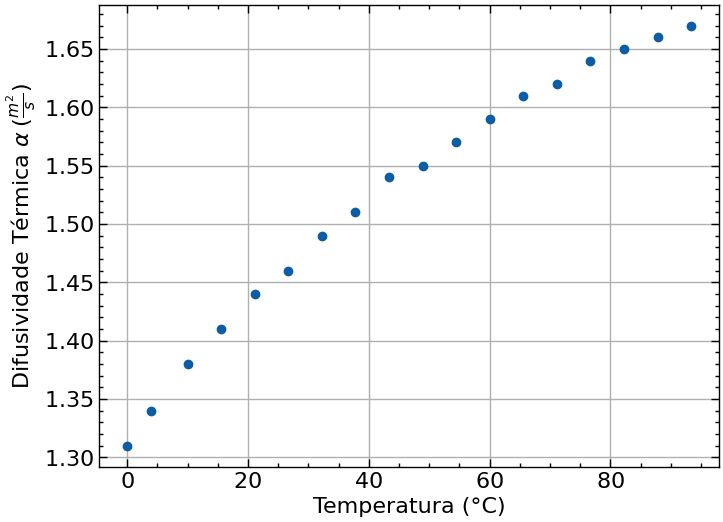
\includegraphics[width=0.8\textwidth]{difusividade_ex1}
    \caption{Gráfico dos dados experimentais}
    \label{fig:grafico_dif_ex1}
\end{figure}
Ao visualizar o gráfico, podemos perceber que os dados parecem estar em uma parábola, então vamos
tentar ajustar uma parábola aos dados. Para isso, vamos utilizar o método dos mínimos quadrados,
com o seguinte código:
\begin{minted}{python}
    import numpy as np
    from scipy.optimize import curve_fit

    T = np.array([0, 4, 10, 15.6, 21.1, 26.7, 32.2, 37.8, 43.3,
        48.9, 54.4, 60, 65.6, 71.1, 76.7, 82.2, 87.8, 93.3])
    alpha = np.array([1.31, 1.34, 1.38, 1.41, 1.44, 1.46, 1.49, 1.51,
        1.54, 1.55, 1.57, 1.59, 1.61, 1.62, 1.64, 1.65, 1.66, 1.67])

    def func(T, a, b, c):
        return a * T**2 + b * T + c

    popt, pcov = curve_fit(func, T, alpha)
    print(popt)

    plt.plot(T, alpha, 'o')
    plt.plot(T, func(T, *popt), 'r-')
    plt.xlabel(r'Temperatura ($\degree C)$')
    plt.ylabel(r'Difusividade Térmica $ \alpha \; (\frac{{m^2}}{{s}})$')
    plt.grid()
    plt.show()
\end{minted}
Onde a função \texttt{func} é a função que representa a parábola, e \texttt{popt} é um vetor que
contém os coeficientes da parábola. O resultado obtido foi:
\begin{minted}{python}
    [-2.48992854e-05  6.08503806e-03  1.31723970e+00]
\end{minted}
Note a falta do \(10^7\), nos valores. O correto é dividir todos os coeficientes por esse fator de
escala. O gráfico obtido foi:
\begin{figure}[H]
    \centering
    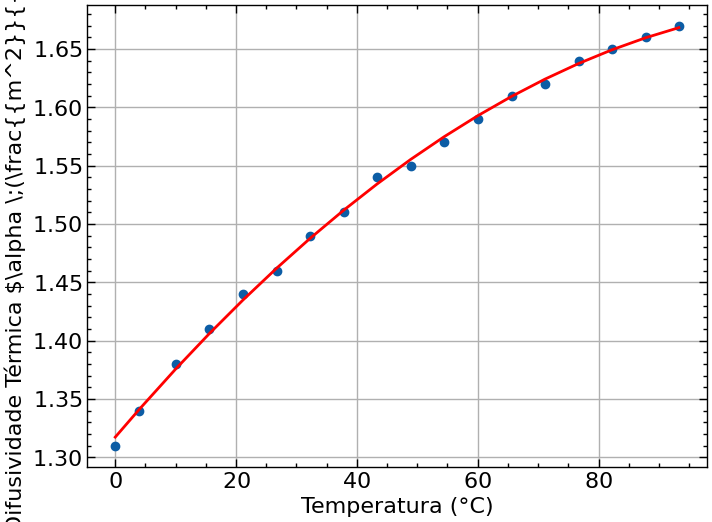
\includegraphics[width=0.8\textwidth]{difusividade_ex1_ajustada}
    \caption{Gráfico dos dados experimentais ajustados}
    \label{fig:grafico_dif_ex1_ajustado}
\end{figure}
Portanto, a função que representa a difusividade térmica da água em função da temperatura é:
\begin{equation}
    \alpha = 1.32 \cdot 10^{-7} + 6.11 \cdot 10^{-10} T - 2.48 \cdot 10^{-12} T^{2}
\end{equation}
\subsection{Densidade}
A densidade é uma propriedade física que relaciona a massa de um material com o seu volume. A
densidade é uma propriedade intensiva, ou seja, não depende da quantidade de matéria presente.
Ela é definida como:
\begin{equation}
    \rho = \frac{m}{V}
\end{equation}
Os métodos de determinação são experimentais, por tabelas ou gráficos, por equações empíricas ou
valores semelhantes. A equação empírica mais utilizada é a equação de Choi e Okos:
\begin{equation}
    \rho = \frac{1}{\sum_{i} \left( X_i^{m}/\rho _{i}   \right) }
\end{equation}
Onde \(X_i\) é a fração mássica do componente \(i\), \(\rho _{i}\) é a densidade do componente \(i\).
\section{Introdução a Condutores de calor}
Trocadores de calor são equipamentos que tem como função transferir calor de um fluido para outro,
seja para resfriamento, seja para aquecimento. Eles são amplamente utilizados em processos
industriais, como em refinarias, usinas de açúcar e álcool, usinas nucleares, etc. Eles podem ser
classificados de acordo com a direção do fluxo dos fluidos, de acordo com o número de fluidos
envolvidos, etc. \par

O ponto de referência que temos é o fluido principal, onde é ele que vamos ter que prestar mais
atenção. Vamos estudar 3 tipos de trocadores de calor, principalmente para seu dimensionamento, que
serão o trocador tubo duplo, o trocador casco e tubos e o trocador de placas. \par

\section{Trocador Tubo Duplo}
Composto por 2 tubos concêntricos, geralmente com 2 trechos retos, com conexões que permitem o
movimento do fluido de uma seção para outra. O conjunto no todo em forma de U é denominado de
grampo. Na parte curva do trocado de calor, não há troca de calor entre os fluídos, sendo
desconsideradas na análise. \par

O fluidos podem operar em contracorrente ou em corrente paralela. Onde em contracorrente é mais
utilizado por gerar trocadores com áreas menores. As vantagens desses trocadores incluem sua
facilidade de construção e montagem, facilidade de ampliação, manutenção, etc. \par

Os tubos concêntricos conduzem duas correntes, cada um com um coeficiente convectivo diferente e com
temperaturas de entrada e saída distintas. Geralmente, a fim de estabelecer a diferença de
temperatura entre o fluido quente \(T\) e o fluido frio \(t\) é necessário levar em conta todas as
resistências entre a temperaturas. \par

Nesse tipo de trocador de calor as resistências encontradas são as da resistências do fluido,
resistência da parede do tubo e a resistência do fluido anelar, ou seja:
\begin{equation}\label{eq:resistencia_tubo_duplo_geral }
    \frac{1}{U} = \sum_{i} R_{i}  =\frac{1}{h_1} + \frac{L}{K} + \frac{1}{h_0}
\end{equation}
Onde \(U\) é o coeficiente global de transferência de calor. Para um tubo com parede grossa, nossa
equação fica
\begin{equation}\label{eq:resistencia_tubo_duplo_parede_grossa_externo }
    \frac{1}{U_{ext}} = \frac{1}{h_{int}} + \frac{D_{ext} }{D_{int}} + \frac{1}{2} \frac{D_{ext} }{K} \ln \frac{D_{ext} }{D_{int}} + \frac{1}{h_{ext}}
\end{equation}
Ou, em relação ao interno:
\begin{equation}\label{eq:resistencia_tubo_duplo_parede_grossa_interno }
    \frac{1}{U_{int}} = \frac{1}{h_{int}} + \frac{1}{2} \frac{D_{int}}{K} \ln \frac{D_{ext} }{D_{int}} + \frac{1}{h_{ext}}\frac{D_{int }}{D_{ext} }
\end{equation}
A transferência de calor por combinação da condução e convecção pode ser dada em relação ao
coeficiente global de transferência de calor:  
\begin{equation}\label{troca_de_calor_U}
    q = UA \Delta T
\end{equation}
Onde \(A\) é a área de troca de calor, \(\Delta T\) é a diferença de temperatura entre as correntes
para toda superfície \(A\). \par

O perfil de temperatura se difere quando falamos de correntes opostas ou em correntes paralelas.
Pelo gráfico abaixo podemos ver a diferença entre os dois perfis:
\begin{figure}[H]
    \centering
    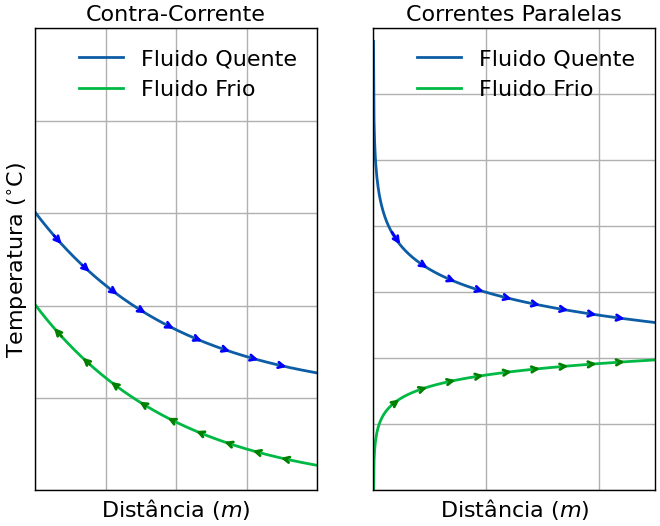
\includegraphics[width=0.8\textwidth]{diferenca_correntes}
    \caption{Diferença entre correntes paralelas e contracorrentes}
    \label{fig:diferenca_correntes}
\end{figure}
\subsubsection{Fatores de Incrustação}
Os fatores de incrustação são fatores que levam em conta a sujeira que pode se acumular na parede
dos tubos, diminuindo a área de troca de calor. Ocorre um aumento da resistência térmica, diminuindo
o desempenho térmico do trocador. \par

A formação de incrustações pode ser causado por diversos fatores, como a corrosão, sedimentação,
cristalização, dentre outros, todos que dependem do tipo de fluido e as características de
escoamento. \par

Incrustações na parte interna e externa do nosso tubo causará um acréscimo de duas resistências, que
deverão ser adicionadas na equação \ref{eq:resistencia_tubo_duplo_geral}, equação que passará a ser
chamada de equação limpa. Nossa equação ficará:
\begin{equation}\label{eq:resistencia_tubo_duplo_incrustado}
    \frac{1}{U_{d}} = \frac{1}{h_{int}} + \frac{1}{h_{ext}} + R_{di} + R_{de} 
\end{equation}
%────────────────────────────────────────────────────────────────────────────────────────────────────────────────────────────────────────────────────
\subsection{Exemplo}
Deseja-se aquecer \(4000 \;\frac{kg}{h}\) de suco de laranja de 26 para 42 \(^{\circ}C\) utilizando  
\(5000 \; \frac{kg}{h}\) de água quente à \(72 \; \degree C\). Um fator de incrustação de \(0.0001
\; h m^{2} \degree \frac{C}{kcal}\) pode ser disponível para cada corrente. Além disso, a pressão
permitida para cada corrente é de \(1 \; \frac{kgf}{cm^{2}}\). Dispõe-se de um certo número de tubos
anulares de 6 metros com tubos IPS de diâmetro nominal de \(2^{\prime \prime} \; x \;
1^{\frac{1}{4}^{\prime \prime} } \). Quantos metros de tubos são necessários? \par

\subsubsection{Primeira Solução}
Para a primeira forma de solução, vamos utilizar o método de Kern. Primeiro fazer o balanço de
energia
\begin{align}
    \dot{M}C_{p} \Delta T &= \dot{m}  c_p \Delta t \\
    T_2 = T_1 - \frac{\dot{M} C_p \Delta T}{\dot{m}c_{p}}
\end{align}
Vamos precisar das propriedades termofísicas na temperatura média, que será
\begin{align}
    \overline{T}_{suco} = \frac{T_1 + T_2}{2} = \frac{26 + 42}{2} = 34 \; ^{\circ}C \\
    \overline{T}_{\acute{a}gua} = \frac{T_1 + T_2}{2} = \frac{72 + 28}{2} = 50 \; ^{\circ}C
\end{align}
Onde o \(28\degree C\) foi um chute aleatório. De acordo com a apostila, o suco de laranja \(11
\degree \) Brix possui as seguintes propriedades:
\begin{align}
    C_{p} &= 3.89 \; \frac{kJ}{kg \; ^{\circ}C} \\
    K &= 0.554 \; \frac{W}{m \; ^{\circ}K}\\
    \rho &= 1.043 \; \frac{kg}{m^{3}} \\  
\end{align}
Sendo ele um fluído não newtoniano, temos também que
\begin{align}
    k &= 0.05 \; Pa.s^{n} \\
    n &= 0.8
\end{align}
Para a água, temos
\begin{align}
    C_{p} &= 4180.7 \; \frac{kJ}{kg \; ^{\circ}C} \\
    K &= 0.64 \; \frac{W}{m \; ^{\circ}C}\\
    \rho &= 998.037 \; \frac{kg}{m^{3}} \\
    \mu &= 0.546 \cdot 10^{-3} \; Pa.s
\end{align}
Com isso, conseguimos a temperatura final da água:
\begin{align}
    T_2 &= T_1 + \frac{\dot{M} C_p \Delta T}{\dot{m}c_{p}} \\
    T_2 &= 72 - \frac{4000 \cdot 3890 \cdot (42 - 26)}{5000 \cdot 4180.7} \\
    T_2 &= 60 \; ^{\circ}C
\end{align}
Agora, vamos recalculas as propriedades da água na temperatura média:
\begin{align}
    \overline{T}_{\acute{a}gua} &= \frac{T_1 + T_2}{2} = \frac{72 + 60}{2} = 66 \; ^{\circ}C 
\end{align}
Como as propriedades não se alteraram muito, esse processo de iteração pode ser feito apenas uma vez
sendo assim, satisfatório. \par

Vamos agora calcular a \(MLDT\). O trocador de calor é de correntes opostas, então
\begin{align}
    MLDT &= \frac{\Delta T_2 - \Delta T_1}{\ln \frac{\Delta T_2}{\Delta T_1}} \\  
    &= \frac{4}{\ln \frac{34}{30}}\\
    &= 31.96 \; ^{\circ}C
\end{align}
Agora, vamos calcular o número de Reynolds para o fluido quente, no ânulo:
\begin{align}
    Re &= \frac{\rho \upsilon D_{eq} }{\mu }
\end{align}
Onde os diâmetros dos tubos, ao quadrado, são
\begin{align}
    D_{int}^{2^{\prime\prime}} = 0.0545 \; m^{2} \\
    D_{ext}^{1 \frac{1}{4}^{\prime \prime}} = 0.0421 \; m^{2}\\
    D_{ext}^{2^{\prime\prime}} = 0.0603 \; m^{2}  
\end{align}
A velocidade pode ser dada por
\begin{align}
    \upsilon &= \frac{\dot{m}}{\rho A} \\
    &= \frac{5000 \cdot 1/3600}{\pi/4 \left[ \left( 0.0525 \right) ^{2} - \left( 0.0421 \right) ^{2}  \right] 998.037}\\
    &= 1.8 \frac{m}{s}
\end{align}
O número de Reynolds é então
\begin{align}
    Re &= \frac{998.037 \cdot 1.8 \cdot 0.0104}{0.546 \cdot 10^{-3}}\\
       & = 34218
\end{align}
O que caracteriza um regime turbulento. \par

Agora, vamos calcular o \(h_{parede,\acute{a}gua}\). Para isso, vamos calcular o número de Nusselt
\begin{align}
    Pr &= \frac{C_p \mu}{K} = (4180 \cdot 0.546 \cdot 10^{-3})/0.64 = 3.57\\
    Nu &= \frac{hD}{K} = 0.023 Re^{0.8} Pr^{0.33} \left( \frac{\mu_b}{\mu _{b} } \right)  \\
    &= 0.023 \cdot 34218^{0.8} \cdot 3.57^{0.33} \left( \frac{0.546 \cdot 10^{-3}}{0.546 \cdot 10^{-3}} \right)  \\
    &= 149\\
    149 &= \frac{hD}{K} \\
    h &= \frac{149 \cdot 0.64}{0.0104} = 9169.2 \; \frac{W}{m^{2} \; ^{\circ}C}
\end{align}
Similarmente, vamos fazer o mesmo para o suco. Primeiro o número de Reynolds
\begin{align}
    Re &= \frac{\rho \upsilon ^{2-n} D^{n} }{8^{n-1} K} \left( \frac{4n}{3n + 1} \right)^{n} \\
\end{align}
Com diâmetros e velocidades
\begin{align}
    D_{int}^{1 \frac{1}{4}^{\prime \prime}} &= 0.035 \;\\
    D_{ext}^{1 \frac{1}{4}^{\prime \prime}} &= 0.0421 \;\\
    \upsilon &= \frac{\dot{m}}{\rho A} \\
    &= \frac{4000 \frac{1}{3600}}{\frac{\pi}{4}\left( 0.035 \right)^{2} 1043 }\\
    &= 1.1 \frac{m}{s}
\end{align}
Por fim, como já colocado, \(n = 0.8\) e \(K = 0.05 \; Pa.s^{n}\), temos
\begin{align}
    Re &= \frac{1043 \cdot 1.1^{2-0.8} \cdot 0.035^{0.8} }{8^{0.8-1} \cdot 0.05} \left( \frac{4 \cdot 0.8}{3 \cdot 0.8 + 1} \right)^{0.8} \\
    &= 2310.9
\end{align}
Sendo considerado regime laminar. Agora, vamos calcular o número de Nusselt, para depois calcularmos
o \(h_{parede_suco}\)
\begin{align}
    Nu &= \frac{hD}{K} = 1.75 \delta ^{\frac{1}{3}} G_{z}^{\frac{1}{3}} \left( \frac{\rho _{b} }{\rho _{p} } \right) \\
    \delta &= \frac{3n+1}{4n} = (3 \cdot 0.8 + 1)/(4 \cdot 0.8) = 1.06 \\
\end{align}
O \(G_{z} \) é o número de Graetz para convecção forçada de fórmula
\begin{align}
    G_{z} &= \frac{\dot{m}C_{p} }{KL}\\
    &=\frac{4000 \frac{1}{3600} 3890}{0.554}\\
    &= 1300.8
\end{align}
Temos também que:
\begin{align}
    \left( \frac{\rho _{b} }{\rho _{p} } \right) &= \frac{K_{b} 8^{n-1} }{K_{p} 8^{n-1} }\\
    &= 1
\end{align}
Calculando então o número de Nusselt
\begin{align}
    Nu &= 1.75 \cdot 1.06^{1/3} \cdot 1300.8^{1/3} \cdot 1^{0.14}\\
    &= 19.4754\\
    19.4754 &= \frac{hD}{K} \\
    h &= \frac{19.4754 \cdot 0.554}{0.035}\\
    &= 308.27 \; \frac{W}{m^{2} \; ^{\circ}C}
\end{align}
Agora, vamos calcular o coeficiente global de transferência de calor
\begin{align}
    U_{ext} &= \left( \frac{1}{h_{par-suco} }\frac{D_{ext}^{tubo int}}{D_{int}^{tubo int} } + \frac{D_{ext}}{2K_{a\textit{\c{c}}o }}\ln \frac{D_{ext}}{D_{int}} + \frac{1}{h{par-\acute{a}gua}}  \right)^{-1}\\
    &= \left( \frac{1}{308.27} \frac{0.0421}{0.035} + \frac{0.0421}{2 \cdot 16.56} \ln \frac{0.0421}{0.035} + \frac{1}{9169.2}  \right)^{-1}\\
    &= \left( 3.90 \cdot 10^{-3} + 2.3478 \cdot 10^{-4} + 1.09 \cdot 10^{-4}  \right)\\
    &= 233.435 \; \frac{W}{m^{2} \; ^{\circ}C}
\end{align}
Adicionando o fator de incrustação, já convertido, vamos ter o fator sujo, dado por:
\begin{align}
    U_{d} &= \frac{1}{U} + 2R_{d}\\
    &= \left(\frac{1}{233.435} + 8.6\cdot 10^{-5}\right)^{-1} \\
    &= 228.841 \; \frac{W}{m^{2} \; ^{\circ}C}
\end{align}
Vamos determinar a área de troca de calor
\begin{align}
    Q &= U_{d}A_{t} MLDT\\
    A_{t} &= \frac{Q}{U_{d}MLDT}\\
    &= \frac{4000 \frac{1}{3600} 3890 \cdot (42-26)}{228.841 \cdot 31.96}\\
    &= 9.4555 \; m^{2}
\end{align}
Agora, vamos achar o comprimento de tubulação
\begin{align}
    L &= \frac{A_{t}}{\pi D_{ext}^{tubo int}}\\
    &= \frac{9.4555}{\pi \cdot 0.0421}\\
    &= 71.4912 \; m
\end{align}
Precisamos determinar a perda de carga no tubo, tanto para a água, tanto para o suco. Como o tubo é
liso, de aço inox, nosso fator de atrito vale \(0.0225\). Nossa formula de perda de carga é, com o
cálculo para a água
\begin{align}
    \frac{\Delta P}{\rho } &= \frac{fL_{eq} }{D} \frac{\upsilon ^{2}}{2}\\
    \Delta P &= \frac{fL_{eq} }{D} \frac{\upsilon ^{2}}{2} \rho\\
    &= 0.0225 \frac{71.4912}{0.0104} \frac{1.8^{2}}{2} 998.037\\
    &= 250071.0527 \; \frac{N}{m^{2} } \cdot \frac{kg}{9.807\;N}\cdot \frac{m^{2} }{100cm^{2}}\\
    &= 2.55 \; kgf/cm^{2}
\end{align}
E para o suco
\begin{align}
    \frac{\Delta P}{\rho } &= \frac{64}{Re}\frac{L}{D}\frac{\upsilon^{2}}{2}\\
    \Delta P &= \frac{64}{Re}\frac{L}{D}\frac{\upsilon^{2}}{2} \rho\\
    &= \frac{64}{2310.9}\frac{71.4912}{0.035}\frac{1.1^{2}}{2} 1043\\
    &= 35696.2872 \; \frac{N}{m^{2} } \cdot \frac{kg}{9.807\;N}\cdot \frac{m^{2} }{100cm^{2}}\\  
    &= 0.364 \; kgf/cm^{2}
\end{align}
O número de tubos é dado por
\begin{align}
    N_{t} &= \frac{71.4912}{6}\\
    &=11.9152 \approx 12
\end{align}
Agora, por fim, vamos determinar as perdas de retorno e as perdas finais. A perda de retorno é dada
por
\begin{align}
    \Delta P_{ret} &= 4 \cdot \left( \frac{\upsilon^{2}}{2}  \right) \rho \\
    \Delta P_{ret, \acute{a}gua} &= 4 \cdot \left( \frac{1.8^{2}}{2}  \right) 998.037 \cdot \frac{1}{9.807 \cdot 100^{2} } =  0.066 \; kgf/cm^{2}\\
    \Delta P_{ret, suco} &= 4 \cdot \left( \frac{1.1^{2}}{2}  \right) 1043 \cdot \frac{1}{9.807 \cdot 100^{2} } = 0.026 \; \frac{kgf}{cm^{2}} \\
\end{align}
Por fim, a perda final é dada por
\begin{align}
    \Delta P_{f, \acute{a}gua} &= \Delta P_{tubo, \acute{a}gua} + \Delta P_{ret,\acute{a}gua}\\
    &= 2.55 + 0.066 \cdot 10\\
    &= 3.21 \; kgf/cm^{2}\\
    \Delta P_{f, suco} &= \Delta P_{tubo, suco} + \Delta P_{ret,suco}\\
    &= 0.364 + 0.026 \cdot 10\\
    &= 0.624 \; kgf/cm^{2}
\end{align}
%────────────────────────────────────────────────────────────────────────────────────────────────────────────────────────────────────────────────────
\section{Trocador Casco-Tubo}
Esse trocador é o mais utilizado na indústria química e de alimentos. Ele é composto por casco,
feixe de tubos, cabeçote móvel ou fixo, bocais e chicana. As funções da chicana é suportar os tubos,
evitando que eles vibrem e quebrem, além de facilitar a transferência de calor e evita regiões
mortas. \par

O espaçamento entre as chicanas é padronizado pelas normas, que definem um valor máximo e mínimo. O
maior número de chicanas aumenta o coeficiente de troca de calor, porém, pode levar a um aumento do
número de vazamentos na corrente principal do casco. O tipo mais comum de chicana é a segmentar \par

Durante o projeto do trocador, é necessário escolher o fluido que escoara pelo lado do casco e pelo
lado dos tubos. Alguns critérios de escolha envolvem a incrustação, corrosão, pressão, viscosidade,
coeficiente de troca de calor, vazão, etc. \par

Quando vamos calcular o diâmetro, precisamos considerar o diâmetro equivalente. Para o lado carcaça
passa quatro, temos: 
\begin{equation}\label{eq:diamentro_equivalente_carcaça_4}
    D_{eq} = \frac{4 \; \textit{Área de escoamento}}{\textit{Perímetro molhado}} = \frac{4 \left( P_{T}^{2} - \pi \frac{D_0 ^{2} }{4} \right)}{\pi D_0 } 
\end{equation}
Onde \(P_{T}\) é o pitch. Para um passe triangular, nossa formula fica
\begin{equation}\label{eq:diamentro_equivalente_carcaça_3}
    D_{eq} = \frac{4 \left( \frac{1}{2} P_{t} \cdot 0.86P_{T} - \frac{1}{2} \pi \frac{D_0 ^{2} }{4} \right)}{\frac{\pi}{2}D_0 \cdot N_{t} }
\end{equation}
Onde \(N_{t}\) é o número de tubos. \par

A área de escoamento na carcaça e no tudo é dado por 
\begin{align}
    A_{escoamento, \text{carcaça}} &= \frac{D_{I} c^{\prime} B}{P_{T} }\label{eq:area_escoamento_carcaça}\\
    A_{escoamento, tubo} &= \frac{N_{t} a_t ^{\prime} }{n}\label{eq:area_escoamento_tubo}
\end{align}
Onde \(D_{I}\) é o diâmetro interno da carcaça, \(c^{\prime}\) é o espaçamento entre os tubos,
\(B\) é o espaço entre as chicanas. \(N_{T} \) é o número de tubos, \(a_{t}^{\prime}\) é a área de
escoamento, dado por tabelas, e \(n\) é o número de passes. \par

Existe uma diferença entre a temperatura real de um trocador e a \(MLDT\) calculado. A relação é
dada por

\begin{equation}\label{eq:temp_real_trocador}
    \Delta T_{real} =  MLDT \cdot F_T
\end{equation}
Onde \(F_{T} \) é um fator de correção dado por
\begin{equation}\label{eq:fator_correcao_trocador}
    F_{T} = \frac{\sqrt{R^{2} + 1} \ln \frac{1 - S}{1 - RS}}{\left( R -1 \right) \ln \frac{2 - S\left( R + 1 - \sqrt{R^{2} + 1}  \right) }{2 - S\left( R + 1 + \sqrt{R^{2} + 1}  \right) }}
\end{equation}
Com \(S\), \(R\) dado por
\begin{align}
    R &= (T_1 - T_2)/(t_2 - t_1)\\
    S &= (t_2 - t_2)/(T_1 - t_1)
\end{align} 

Esse valor é tabelado, geralmente em função de \(R\) e \(S\), onde serão olhados graficamente. \par

\begin{figure}[H]
\centering
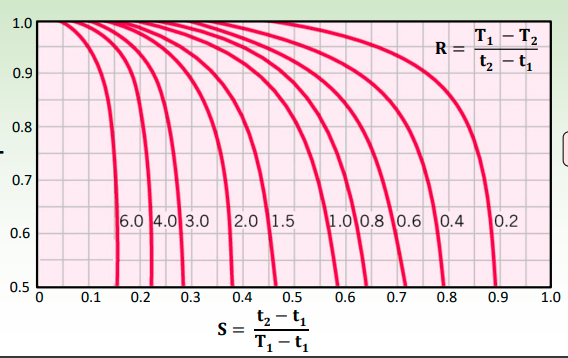
\includegraphics[width=0.8\textwidth]{R_S_Grafico}
\caption{Gráfico de \(R\) e \(S\) para o fator de correção \(F_{T}\)}
\label{fig:R_S_Grafico}
\end{figure}

A queda de pressão no lado da carcaça é dada por

\begin{equation}\label{eq:queda_pressao_carcaça}
    \frac{\Delta P_{\text{carcaça}}}{\rho } = f \frac{D_{c} \left( N+1 \right) }{D_{eq} }\frac{\upsilon ^{2} }{2}
\end{equation}
Onde é uma formula modificada da Lei de Darcy. \(N\) é o número de chicanas, \(D_{c}\) é o diâmetro 
da carcaça e \(D_{eq}\) é o diâmetro equivalente. \par

A queda de pressão no interior dos tubos é dada pela Lei de Darcy normal, ou seja:
\begin{equation}\label{eq:queda_pressao_tubo}
    \frac{\Delta P_{tubo}}{\rho } = f \frac{L_{eq} }{D_{eq} }\frac{\upsilon ^{2} }{2}
\end{equation}
Onde \(L_{eq}\) é o comprimento equivalente, que deve ser multiplicado pelo número de passagens.
\par
\subsection{Exemplo}
Numa industria há um trocador de calor tipo carcaça tubo 1:2 com 160 tubos de cobre BWG 18 de
\(\frac{3}{4}^{\prime \prime}\) e comprimento de 5 metros, arranjo triangular, pitch
\(\frac{15}{16}^{\prime \prime} \) com chicanas de espessura \(2.5 \;mm\) espaçadas de \(30 \; cm\).
Necessita-se saber se o trocador será adequado para resfriar \(80000 \; \frac{kg}{h}\) de água
destilada da temperatura de \(35 \; \degree C \to 30 \; \degree C\), dispondo de \(150000 \;
\frac{kg}{h}\) de água não tratada à \(22 \; \degree C\). A perda de carga admissível em cada
corrente é de 10 psi e o fator de incrustação é de \(0.0001 \) e \(0.0003 \; h m^{2} C / kcal\) para
água destilada e não tratada, respectivamente, desde que a velocidade não seja menor que 2 \(\frac{m}{s}\).       
 
\subsubsection{Solução}
Pelo método de Kern, vamos calcular a temperatura de saída do fluído frio. Pelo balanço de energia
temos
\begin{align}
    \dot{M}C_{p} \Delta T &= \dot{m}  c_p \Delta t \\
    t_2 &= t_1 + \frac{\dot{M} C_p \Delta T}{\dot{m}c_{p}}\\
    t_2 &= 22 + \frac{80000 \cdot 1 \cdot \left( 35 - 30 \right) }{150000 \cdot 1}\\
    t_2 &= 24.6667 \; \degree C
\end{align}
De acordo com nosso enunciado, as características do nosso trocador são:
\begin{itemize}
    \item {Carcaça:\\
            \begin{itemize}
            \item L = \(5 \; m\)  \\
            \item D = \(15 \frac{1}{4}^{\prime \prime} \)\\
            \item Passagem = 1\\
            \item Espessura Chicana = \(0.0025 \; m\) \\
            \item \(P_{T} \) = \(0.0238 \; m\) \\
            \item \(C^{\prime} \) = \(P_{T} - D_{e} = 0.00483 \; m\)\\
            \item B = \(0.3 \; m\) \\
            \end{itemize}
    }
    \item {Tubos:\\
            \begin{itemize}
            \item L = \(5 \; m\) \\
            \item \(D_{E}\)  = \(3/4^{\prime \prime} \)\\
            \item Passagem = 2\\
            \item \(D_{I}\) = \(0.0166 \; m\)\\
            \item Arranjo triangular\\
            \item N = 160\\  
            \end{itemize}
    }
\end{itemize}
Agora, vamos pegar as propriedades termofísicas, na temperatura média \(32.5 \; \degree C\) , da água destilada:
\begin{align}
    C_{p} &= 0.998 \; \frac{kJ}{kg \; ^{\circ}C} \\
    K &= 0.53 \; \frac{\mathcal{K} }{h m^{2} \degree C}\\
    \mu &= 0.798 \cdot 10^{-3} \; \frac{kg}{m \cdot s}\\
    \rho &= 995.6 \frac{kg}{m^{3}}
\end{align}
Para a água não tratada (\(23 \degree C\) ), temos:
\begin{align}
    C_{p} &= 0.998 \; \frac{kJ}{kg \; ^{\circ}C} \\
    K &= 0.51 \; \frac{\mathcal{K} }{h m^{2} \degree C}\\
    \mu &= 1 \cdot 10^{-3} \; \frac{kg}{m \cdot s}\\
    \rho &= 996.2 \frac{kg}{m^{3}}
\end{align}
Para calcular a \(MLDT\) temos de levar em conta que como são 2 passes, o primeiro será em
contra-corrente e o segundo em corrente paralela. Para as diferenças, temos \(\Delta T_1 = 35 - 24.7
= 10.3 \; \degree C\) e \(\Delta T_2 = 30 - 22 = 8 \degree C\). Portanto, nossa \(MLDT\) vale
\begin{align}
    MLDT &= \frac{\Delta T_1 - \Delta T_2}{\ln \frac{\Delta T_1}{\Delta T_2}}\\
    &= \frac{10.3 - 8}{\ln \frac{10.3}{8}}\\
    &= 9.1016 \; \degree C   
\end{align}
Agora, teremos que achar o valor verdadeiro de temperatura, primeiro vamos calcular \(S, R\)
\begin{align}
    R &= \frac{35 - 30}{24.7 - 22} = 1.8518 \\
    S &= \frac{24.7 - 22}{35 - 22} = 0.2077 \\
\end{align}
Com isso, vamos achar o fator de correção \(F_{T}\)
\begin{align}
    F_{T} &= \frac{\sqrt{R^{2} + 1} \ln \frac{1 - S}{1 - RS}}{\left( R -1 \right) \ln \frac{2 - S\left( R + 1 - \sqrt{R^{2} + 1}  \right) }{2 - S\left( R + 1 + \sqrt{R^{2} + 1}  \right) }}\\
    &= \frac{\sqrt{1.8518^{2} + 1} \ln \frac{1 - 0.2077}{1 - 1.8518 \cdot 0.2077}}{\left( 1.8518 -1 \right) \ln \frac{2 - 0.2077\left( 1.8518 + 1 - \sqrt{1.8518^{2} + 1}  \right) }{2 - 0.2077\left( 1.8518 + 1 + \sqrt{1.8518^{2} + 1}  \right) }}\\
    &= 0.9721
\end{align}
Ou, graficamente, que é bem mais fácil, chegaríamos num valor de \( \approx 0.97\). Com isso, nossa
temperatura real será
\begin{align}
    \Delta T_{real} &= 9.1016 \cdot 0.9721\\
    &= 8.8477 \; \degree C
\end{align}
Agora, vamos calcular o número de Reynolds para o lado da carcaça. Primeiro vamos precisar da área
de escoamento, que será
\begin{align}
    A_{escoamento, \text{carcaça}} &= \frac{P_{T} ^{2} \cdot 0.866}{2} - \frac{\pi D_{ext} ^{2} }{2 \cdot 4}\\
    &= \frac{0.0238^{2} \cdot 0.866}{2} - \frac{\pi \cdot 0.0191^{2} }{2 \cdot 4}\\
    &= 1.0201 \cdot 10^{-4} \; m^{2}
\end{align}
O perímetro molhado é dado por
\begin{align}
    P_{m} &= \pi \frac{D_{ext}}{2}\\
    &= \pi \frac{0.0191}{2}\\
    &= 0.03 \; m
\end{align}
Agora, nosso diâmetro equivalente é dado por
\begin{align}
    D_{eq} &= \frac{4 \cdot A_{escoamento, \text{carcaça}}}{P_{m} \cdot N}\\
    &= \frac{4 \cdot 1.0201 \cdot 10^{-4}}{0.03 \cdot 160}\\
    &= 8.501 \cdot 10^{-5}
\end{align}
Agora, vamos calcular a área superficial
\begin{align}
    A_{escoamento, \text{carcaça}} &= \frac{D_{I} c^{\prime} B}{P_{T} } \\
    A_{escoamento, \text{carcaça}} &= \frac{0.387 \cdot 0.00483 \cdot 0.3}{0.0238}\\
    &= 0.02356 \; m^{2} 
\end{align}

Agora vamos calcular a velocidade

\begin{align}
    \upsilon &= \frac{\dot{m}}{\rho A_{escoamento, \text{carcaça}}}\\
    &= \frac{80000 \cdot 1/3600}{995.6 \cdot 0.02356}\\
    &= 0.9474 \; \frac{m}{s}
\end{align}
O número de Reynolds é dado por
\begin{align}
    Re &= \frac{\rho \upsilon D_{eq} }{\mu }\\
    &= \frac{995.6 \cdot 0.9474 \cdot 8.501 \cdot 10^{-5}}{0.798 \cdot 10^{-3}}\\
    &= 100.4813
\end{align}
O regime é laminar. Vamos calcular o número de Reynolds para o lado dos tubos. Primeiro, vamos
calcular a velocidade
\begin{align}
    \upsilon &= \frac{\dot{m}}{\rho A_{escoamento, tubo}}\\
    &= \frac{150000 \cdot 1/3600}{996.2 \cdot \frac{\pi \cdot 0.0166^{2} \cdot 160}{4 \cdot 2}}\\
    &= 2.4157 \; \frac{m}{s}
\end{align}
O número de Reynolds é dado por
\begin{align}
    Re &= \frac{\rho \upsilon D_{eq} }{\mu }\\
    &= \frac{996.2 \cdot 2.4157 \cdot 0.0166}{1 \cdot 10^{-3}}\\
    &= 39948.2376
\end{align}
Sendo turbulento. Vamos calcular o número de Proust para o lado tubo:
\begin{align}
    Pr &= \frac{C_{p} \mu}{K}\\
    &= \frac{0.998 \cdot 1 \cdot 10^{-3} \cdot 3600}{0.51}\\
    &= 7.0447
\end{align}
Agora, para o lado carcaça
\begin{align}
    Pr &= \frac{C_{p} \mu}{K}\\
    &= \frac{0.998 \cdot 0.798 \cdot 10^{-3} \cdot 3600}{0.53}\\
    &= 5.4095
\end{align}
Agora, vamos calcular o número de Nusselt para o lado dos tubos
\begin{align}
    Nu &= \frac{hD}{K} = 0.023 \left[ 1 + \left( \frac{D}{L} \right) ^{0.7}  \right] Re^{0.8} Pr^{0.33} \left( \frac{\mu _{b} }{\mu _{p} } \right) ^{0.14}\\
    &= 0.023 \left[ 1 + \left( \frac{0.0166}{5} \right) ^{0.7}  \right] 39948.2376^{0.8} 7.0447^{0.33} \left( \frac{1 \cdot 10^{-3}}{1 \cdot 10^{-3}} \right) ^{0.14}\\
    &= 214.11079 
\end{align}
O coeficiente de transferência de calor é dado por
\begin{align}
    h &= \frac{Nu K}{D}\\
    &= \frac{214.11079 \cdot 0.51}{0.0166}\\
    &= 6578.10258 \; \frac{kcal}{h \cdot m^{2} \; ^{\circ}C}
\end{align}
Agora, vamos calcular o número de Nusselt para o lado da carcaça
\begin{align}
    Nu &= 0.36 \left( \frac{D_{eq} \rho \upsilon }{\mu } \right)^{0.55} \left( \frac{\mu c_{p} }{k} \right)^{\frac{1}{3}} \left( \frac{\mu }{\mu _{p} } \right) ^{0.14}\\
    &= 0.36 \left(\frac{8.501 \cdot 10^{-5} \cdot 995.6 \cdot 0.9474 }{0.798 \cdot 10^{-3}}  \right)^{0.55} \left( \frac{0.798 \cdot 10^{-3} \cdot 4180 }{0.53} \right)^{\frac{1}{3}} \left( \frac{0.798 \cdot 10^{-3} }{0.798 \cdot 10^{-3}} \right) ^{0.14}\\
    &= 8.3898 
\end{align}
%To do, arrumar essa conta
O coeficiente de transferência de calor é dado por
\begin{align}
    h &= \frac{Nu K}{D_{eq}}\\
    &= \frac{8.3898 \cdot 0.53}{8.501 \cdot 10^{-5}}\\
    &= 52306.71686 \; \frac{kcal}{h \cdot m^{2} \; ^{\circ}C}
\end{align}
Vamos determinar o coeficiente global de transferência de calor
\begin{align}
    U_{sujo} &= \left( \frac{1}{h_{i} }\frac{D_E}{D_{i} } + \frac{D_E}{2K} \ln \frac{D_E}{D_{i} } + \frac{1}{he} + R_{di} + R_{dE}  \right)^{-1} \\
    &= \left( \frac{1}{6578.10258} \cdot  \frac{0.0191}{0.0166} + \frac{0.0191}{2 \cdot 342.3} \cdot  \ln \left( \frac{0.0191}{0.0166} \right)  + \frac{1}{52306.71686} + 0.0001 + 0.0003  \right)^{-1}\\
    &= 1672.3920 \; \frac{kcal}{h m^{2} \degree C}\\
\end{align}
A área de troca de calor é dada por
\begin{align}
    A_{t} &= \frac{Q}{U_{sujo} MLDT}\\
    &= \frac{80000 \cdot 1 \cdot \left( 35 - 30 \right) }{1672.3920 \cdot 9.1016}\\
    &= 26.2787 \; m^{2}
\end{align} 
Falta agora descobrir as perdas de carga. Primeiro, vamos calcular para os tubos. Como o tubo é
liso, seu fator de atrito vale \(0.022\). Vamos utilizar a formula de Darcy-Weisbach
\begin{align}
    \frac{\Delta P}{\rho } &= \frac{fL_{eq} }{D} \frac{\upsilon ^{2}}{2}\\
    &= 0.022 \frac{2 \cdot 5}{0.0166} \frac{2.4157^{2}}{2}\\
    &= 38.6697 \; \frac{J}{kg}
\end{align}
Agora, vamos calcular a perda de carga no retorno
\begin{align}
    \left(\frac{\Delta P}{\rho }\right)_{retorno} &= 4 \cdot \left( \frac{\upsilon ^{2}}{2}  \right) \rho \\
    &= 4 \cdot \left( \frac{2.4157^{2}}{2}  \right)\\
    &= 11.6712 \; \frac{m^{2} }{s ^{2} }
\end{align}
A perda total nos tubos é a soma das duas, logo
\begin{align}
    \left(\frac{\Delta P}{\rho }\right)_{tubo} &= 38.6697 + 11.6712\\
    &= 50.3409 \; \frac{m^{2} }{s ^{2} } \cdot 996.2 \frac{kg}{m  ^{3}} \cdot \frac{1.45 \cdot 10^{-4}}{1 \text{pascal}}\\
    &= 7.2716926641 \; psi
\end{align}
Agora, vamos calcular a perda de carga na carcaça. Como o regime é laminar, nosso fator de atrito é
achado pelo gráfico de Moody, que vale \(f = 0.864\). Através da formula de Darcy-Weisbach,
modificada, \eqref{eq:queda_pressao_carcaça}, temos
\begin{align}
    \frac{\Delta P}{\rho } &= f \frac{D_{c} \left( N+1 \right) }{D_{eq} }\frac{\upsilon ^{2} }{2}\\
    &= 0.864 \frac{0.387 \cdot \left( 16 + 1 \right) }{8.501 \cdot 10^{-5}} \frac{0.9474^{2}}{2}\\
    &= 30008.2299 \; \frac{m^{2} }{s ^{2} } \cdot 995.6 \frac{kg}{m  ^{3}} \cdot \frac{1.45 \cdot 10^{-4}}{1 \text{pascal}}\\
    &= 4332.0480848238 \; psi
\end{align}
%Acho que isso ta resolvido

% \chapter{Bioquímica}
\secton{Introdução}
 
% \chapter{Fenômenos de Transporte III}
\section{Introdução a Fundamentos da Transferência de Massa}
\subsection{Definição}
Transferência de massa é aquela massa em trânsito resultante da diferença de concentração de alguma
espécie na mistura. Logo, a diferença de concentração pode ser vista como a força motriz, assim a
diferença de temperatura era a força motriz para transferência de calor. \par

Necessariamente tem que haver uma diferença de concentração para que ocorra movimentação de massas.
Ela pode ocorrer por meio de difusão, onde naturalmente a massa vai migrar de uma região de maior
concentração para aquela de menor, ou por convecção, onde a massa é forçadamente movimentada para a
região de interesse. \par

\section{Concentrações}
\subsection{Concentração mássica}
A concentração mássica é definida como
\begin{equation}\label{eq:conc_massica}
    \rho_i = \frac{m_i}{V}
\end{equation}
Onde \(\rho _{i} \) é a concentração mássica da espécie \(i\), \(m_i\) é a massa da espécie \(i\) e
\(V\) é o volume do sistema. \par
%────────────────────────────────────────────────────────────────────────────────────────────────────────────────────────────────────────────────────

\subsection{Concentração molar}
A concentração molar é definida como
\begin{equation}\label{eq:conc_molar}
    C_i = \frac{n_i}{V} = \frac{\rho _i}{M_i}
\end{equation}
Onde \(C_i\) é a concentração molar da espécie \(i\), \(n_i\) é o número de mols, \(\rho _{i} \) é a
concentração mássica e \(M_{i} \) é a massa molar. \par
%────────────────────────────────────────────────────────────────────────────────────────────────────────────────────────────────────────────────────
\subsection{Fração Mássica}
A fração mássica é definida como
\begin{equation}\label{eq:frac_massica}
    \omega _{i} = \frac{\rho _{i} }{\rho }
\end{equation}
Onde \(\rho = \sum_{i} \rho _{i} \) é a soma das concentrações mássicas de todas as espécies. \par
%────────────────────────────────────────────────────────────────────────────────────────────────────────────────────────────────────────────────────
\subsection{Fração Molar}
A fração molar para líquidos é definida como
\begin{equation}\label{eq:frac_molar_liquidos}
    x _{i} = \frac{C_{i} }{C}
\end{equation}
Para gases é definida como
\begin{equation}\label{eq:frac_molar_gas}
    y _{i} = \frac{C_{i} }{C}
\end{equation}
Em que para ambos \(C = \sum_{i} C_{i} \) é a soma das concentrações molares de todas as espécies.
\par
%────────────────────────────────────────────────────────────────────────────────────────────────────────────────────────────────────────────────────
\subsection{Definições Básicas para Uma Mistura Binária}
Para uma mistura binária, ficam definidos que:
\begin{align}
    \text{Concentração mássica da solução} \quad & \rho = \rho _{a} + \rho _{b} \label{eq:conc_massica_solucao} \\
    \text{Concentração molar da mistura} \quad & C = C_{a} + C_{b} \label{eq:conc_molar_mistura} \\
    \text{Concentração mássica de uma das substâncias} \quad & \rho_{a / b} = C_{a / b} M_{a / b} \label{eq:conc_massica_substancia} \\
    \text{Concentração molar de uma das substâncias} \quad & C_{a / b} = \frac{\rho_{a / b}}{M_{a / b}} \label{eq:conc_molar_substancia} \\
    \text{Concentração molar da mistura} \quad & C = \frac{\rho }{M} \label{eq:conc_molar_mistura_{total}}\\
    \text{Fração mássica de uma das misturas} \quad & \omega _{a / b} = \frac{\rho _{a / b} }{\rho } \label{eq:frac_massica_substancia} \\
    \text{Fração molar de uma das misturas para líquidos} \quad & x_{a / b} = \frac{C_{a / b} }{C} \label{eq:frac_molar_substancia_liq} \\
    \text{Fração molar de uma das misturas para gases} \quad & y_{a / b} = \frac{C_{a / b} }{C} \label{eq:frac_molar_substancia_gas}
\end{align}
Algumas relações adicionais são:
\begin{align}
    \omega _{a} + \omega _{b} = 1 \label{eq: relacao_frac_massica} \\
    \frac{\omega _{a} }{M_{a} } + \frac{\omega _{b} }{M_{b} } = \frac{1}{M} \label{eq:relacao_frac_massica_massa_molar} \\
    \omega _{a} = \frac{x_{a} M_{a} }{x_{a} M_{a} + x_{b} M_{b} } \label{eq:relacao_frac_massica_frac_molar} \\
    x_{a} + x_{b} = 1 \label{eq:relacao_frac_molar_liq} \\
    y_{a} + y_{b} = 1 \label{eq:relacao_frac_molar_gas} \\
    x_{a} M_{a} + x_{b} M_{b} = M \label{eq:relacao_frac_molar_massa_molar} \\
    x_{a} = \frac{\frac{\omega _{a} }{M_{a} } }{\frac{\omega _{a} }{M_{a} } + \frac{\omega _{b} }{M_{b} } } \label{eq:relacao_frac_molar_frac_massica} \\
\end{align}
%────────────────────────────────────────────────────────────────────────────────────────────────────────────────────────────────────────────────────
\subsection{Exemplo 1}\label{subsec:ex1}
Determine o peso molecular da mistura abaixo:
\begin{table}[H]
\centering
\begin{tabular}{c|c|c}
\toprule
Componente & Peso Molecular &  y \\
 \midrule
 CO & 28 &  0.05 \\
 \ch{H20} & 18 &  0.20 \\
 \ch{O2} & 32 &  0.04 \\
 \ch{N2} & 28 &  0.71 \\
\bottomrule
\end{tabular}
\caption{Componentes da Mistura}
\label{tab:comp_mist_ex1}
\end{table}
\subsubsection{Solução}
O peso molecular é dado pela seguinte formula:
\begin{equation}
    M = \sum_{i} y_{i} M_{i}
\end{equation}
Logo, vamos ter:
\begin{align}
    M &=  0.05 \cdot 28 + 0.20 \cdot 18 + 0.04 \cdot 32 + 0.71 \cdot 28 \\
    M &= 26.16 \; \frac{g}{mol}
\end{align}
Para achar a fração mássica de cada componente, vamos usar a seguinte formula:
\begin{equation}
    \omega _{i} = \frac{y_{i} M_{i} }{M}
\end{equation}
Logo, vamos ter:
\begin{align}
    \omega _{CO} &= \frac{0.05 \cdot 28}{26.16} = 0.053 \\
    \omega _{\ch{H2O}} &= \frac{0.20 \cdot 18}{26.16} = 0.138 \\
    \omega _{\ch{O2}} &= \frac{0.04 \cdot 32}{26.16} = 0.049 \\
    \omega _{\ch{N2}} &= \frac{0.71 \cdot 28}{26.16} = 0.760
\end{align}
%────────────────────────────────────────────────────────────────────────────────────────────────────────────────────────────────────────────────────
\subsection{Exemplo 2}
Calcule a fração molar de cada espécie, da mistura abaixo:
\begin{table}[H]
\centering
\begin{tabular}{c|c}
\toprule
Componente &  \% mássica \\
 \midrule
 \ch{O2} &  16 \\
 \ch{CO} &  4 \\
 \ch{CO2}  &  17 \\
 \ch{N2} &  63 \\
\bottomrule
\end{tabular}
\caption{Mistura Exemplo 2}
\label{tab:mist_tab_ex2}
\end{table}
\subsubsection{Solução}
Para calcularmos a fração molar de cada espécie, vamos usar a seguinte formula:
\begin{equation}
    y_{i} = \frac{\omega _{i} M}{M_{i} }
\end{equation}
Portanto, vamos calcular \(M\):
\begin{align}
    M &=  \omega _{O_{2}} M_{O_{2}} + \omega _{CO} M_{CO} + \omega _{CO_{2}} M_{CO_{2}} + \omega _{N_{2}} M_{N_{2}} \\
    &=  0.16 \cdot 32 + 0.04 \cdot 28 + 0.17 \cdot 44 + 0.63 \cdot 28 \\
    &=  31.36 \; \frac{g}{mol}
\end{align}
Por fim, vamos calcular as frações molares:
\begin{align}
    y_{O_{2}} &= \frac{0.16 \cdot 31.36}{32} = 0.156 \\
    y_{CO} &= \frac{0.04 \cdot 31.36}{28} = 0.045 \\
    y_{CO_{2}} &= \frac{0.17 \cdot 31.36}{44} = 0.121 \\
    y_{N_{2}} &= \frac{0.63 \cdot 31.36}{28} = 0.678
\end{align}
%────────────────────────────────────────────────────────────────────────────────────────────────────────────────────────────────────────────────────
\section{Velocidades}
A velocidade média das espécies é a médias das velocidades de cada espécie, ponderadas sobre o valor
que queremos, ou seja:
\begin{equation}\label{eq:velocidade_media_massica}
    \overline{\upsilon } = \frac{\sum_{i} \rho _{i} \overline{\upsilon }_{i} }{\sum_{i} \rho _{i} }
\end{equation}
Onde essa é a velocidade média mássica pois está ponderada sobre a massa das espécies. Já a
velocidade média molar é dada por:
\begin{equation}\label{eq:velocidade_media_molar}
    \overline{\Upsilon } = \frac{\sum_{i} C_i \overline{\upsilon }_{i} }{\sum_{i} C_i }
\end{equation}
Onde temos que as quantidades \(C_{i} \overline{\upsilon }, \; \rho _{i} \overline{\upsilon } _{i}
\) são as velocidades locais a qual a massa atravessa uma seção unitária. Essas velocidades pode
estar associadas a outros tipos de velocidade, como a velocidade dos eixos estacionários
\(\overline{\upsilon } = 0\) ou à velocidade de solução \(\overline{\upsilon } _{i} -
\overline{\upsilon } \), para a mássica e \(\overline{\upsilon } _{i} - \overline{\Upsilon } \) para
a molar. Podemos pensar nelas como a velocidade de difusão das nossas massas, ou seja, a velocidade
das espécias relativas à solução.
%────────────────────────────────────────────────────────────────────────────────────────────────────────────────────────────────────────────────────
\subsection{Exemplo 3}
Sabendo que as velocidades médias das espécies do exemplo 1 são:
\begin{table}[H]
\centering
\begin{tabular}{c|c|c}
\toprule
Espécie & Velocidade (\(\frac{cm}{s}\) ) &  y \\
 \midrule
 \ch{CO} &  10 &  0.05 \\
 \ch{H2O} & 19 & 0.20  \\
 \ch{O2} & 13 &  0.04 \\
 \ch{N2} & 11 & 0.71  \\
\bottomrule
\end{tabular}
\caption{Velocidade médias das espécies}
\label{tab:vel_med_tab}
\end{table}
Calcule:
\begin{enumerate}
    \item Velocidade Média Molar da Mistura \label{item:ex3_q1}
    \item Velocidade Média Mássica da Mistura \label{item:ex3_q2}
    \item Velocidade de difusão de cada espécie na mistura, tendo em conta a velocidade molar da mistura \label{item:ex3_q3}
    \item Velocidade de difusão de cada espécie na mistura, tendo em conta a velocidade mássica da mistura \label{item:ex3_q4}
\end{enumerate}
\subsubsection{Solução}
\ref{item:ex3_q1} Tendo em conta que \(M = 26.16 \; \frac{g}{gmol}\) conseguimos calcular a
velocidade média molar da mistura
\begin{align}
    \overline{\Upsilon } &= \frac{\sum_{i} C_i \overline{\upsilon }_{i} }{\sum_{i} C_i }\\
    & = \sum_{i} y_{i} \overline{\upsilon }_{i} \\
    & = 0.05 \cdot 10 + 0.20 \cdot 19 + 0.04 \cdot 13 + 0.71 \cdot 11 \\
    & = 12.63 \; \frac{cm}{s}
\end{align}
\ref{item:ex3_q2} Para calcularmos a velocidade média mássica da mistura, vamos usar a equação
\ref{eq:velocidade_media_massica}:
\begin{align}
    \overline{\upsilon } &= \frac{\sum_{i} \rho _{i} \overline{\upsilon }_{i} }{\sum_{i} \rho _{i} } \\
    & = \sum_{i} \omega _{i} \overline{\upsilon } _{i} \\
    & = 0.054 \cdot 10 + 0.138 \cdot 19 + 0.049 \cdot 13 + 0.759 \cdot 11 \\
    & = 12.148 \; \frac{cm}{s}
\end{align}
\ref{item:ex3_q3} Para calcularmos a velocidade de difusão de cada espécie na mistura, em relação à
velocidade molar da mistura, vamos apenas subtrair a velocidade da espécie pela velocidade média molar
\begin{align}
    \overline{\upsilon } _{i} - \overline{\Upsilon } &= 10 - 12.63 = -2.63 \\
    \overline{\upsilon } _{i} - \overline{\Upsilon } &= 19 - 12.63 = 6.37 \\
    \overline{\upsilon } _{i} - \overline{\Upsilon } &= 13 - 12.63 = 0.37 \\
    \overline{\upsilon } _{i} - \overline{\Upsilon } &= 11 - 12.63 = -1.63
\end{align}
\ref{item:ex3_q4} Para calcularmos a velocidade de difusão de cada espécie na mistura, em relação à
velocidade mássica da mistura, vamos apenas subtrair a velocidade da espécie pela velocidade média
mássica
\begin{align}
    \overline{\upsilon } _{i} - \overline{\upsilon } &= 10 - 12.148 = -2.148 \\
    \overline{\upsilon } _{i} - \overline{\upsilon } &= 19 - 12.148 = 6.852 \\
    \overline{\upsilon } _{i} - \overline{\upsilon } &= 13 - 12.148 = 0.852 \\
    \overline{\upsilon } _{i} - \overline{\upsilon } &= 11 - 12.148 = -1.148
\end{align}
%────────────────────────────────────────────────────────────────────────────────────────────────────────────────────────────────────────────────────
\section{Fluxos} 
O fluxo de uma espécie é definido como a quantidade de massa que atravessa uma seção unitária por
unidade de tempo. Para uma determinada espécie \(i\) o fluxo é dado por:
\begin{equation}\label{eq:fluxo}
    J = \upsilon C
\end{equation}
Onde \(\upsilon \) é a velocidade média da espécie \(i\) e \(C\) é a concentração da espécie. Se
imaginarmos um rio, com vários peixes nadando, a velocidade de um cardume vai ser determinado pela
contribuição que o rio tem, mais a velocidade do peixe. Ou seja, a velocidade de fluxo mais a
velocidade do próprio peixe. Logo, podemos escrever a contribuição do difusiva, ou seja, a
velocidade da espécie como:
\begin{equation}\label{eq:contribuição_espécie}
    J_{a,z} = C_a(\upsilon_{a,z} + \Upsilon_{z} )
\end{equation}
Onde \(J_{a,z}\) é o fluxo da espécie \(a\) na direção \(z\), \(C_a\) é a concentração da espécie \(a\),
\(\upsilon_{a,z}\) é a velocidade da espécie \(a\) na direção \(z\) e \(\Upsilon_{z}\) é a
velocidade de fluxo na direção \(z\). Para a velocidade do fluxo, temos que:
\begin{equation}\label{eq:contribuição_fluxo}
    J_{a,z}^C =  C_{a} \Upsilon _{z} 
\end{equation}
Onde por fim, nossa equação de fluxo fica:
\begin{equation}\label{eq:fluxo_final}
    N_{a,z} = J_{a,z} + J_{a,z}^C = C_a(\upsilon_{a,z} + \Upsilon_{z} ) + C_{a} \Upsilon _{z}
\end{equation}
Onde temos algumas notações de índices, colocadas na tabela abaixo
\begin{table}[H]
\centering
\begin{adjustbox}{width=1\textwidth, center=\textwidth}
\begin{tabular}{c|c|c|c}
\toprule
Velocidade Mássica  & Velocidade média Mássica & Velocidade Molar & Velocidade média Molar  \\
 \midrule
\(J_{a,z} = C_a(\upsilon_{a,z} - \Upsilon_{z} )\)   & \(J_{a,z}^{\star}  = C_a(\upsilon_{a,z} - \upsilon_{z} )\)  & \(j_{a,z} = \rho _a(\upsilon_{a,z} - \Upsilon_{z} )\)   & \(j_{a,z}^{\star}  = \rho _a(\upsilon_{a,z} - \upsilon_{z} )\)  \\
\(J_{a,z}^C =  C_{a} \Upsilon _{z}\)   & \(J_{a,z}^{\star C}  =  C_{a} \upsilon _{z} \)   &  \(j_{a,z}^C =  \rho _{a} \Upsilon _{z}\)   & \(j_{a,z}^{\star C}  =  \rho _{a} \upsilon _{z} \)\\
\(N_{a,z} =C_a(\upsilon_{a,z} - \Upsilon_{z} ) + C_{a} \Upsilon _{z}\)   & \(N_{a,z}^{\star} = C_a(\upsilon_{a,z} - \upsilon_{z} ) + C_{a} \upsilon _{z}\) &  \(n_{a,z} = \rho _a(\upsilon_{a,z} - \Upsilon_{z} ) + \rho _{a} \Upsilon _{z}\)   & \(n_{a,z}^{\star} = \rho _a(\upsilon_{a,z} - \upsilon_{z} ) + \rho _{a} \upsilon _{z}\)\\
\bottomrule
\end{tabular}
\end{adjustbox}
\caption{Notações de índices}
\label{tab:not_indices}
\end{table}
%────────────────────────────────────────────────────────────────────────────────────────────────────────────────────────────────────────────────────
\subsection{Exemplo}
Sabendo que a mistura da \ref{subseq:ex1} está a \(105 \; \degree C\) e a pressão de \(1 \; atm\),
calcule 
\begin{enumerate}
    \item O fluxo difusivo molar de cada espécie \label{item:ex4_q1}
    \item O fluxo difusivo mássico de cada espécie \label{item:ex4_q2}
    \item A contribuição do fluxo convectivo molar de cada espécie \label{item:ex4_q3}
    \item A contribuição do fluxo convectivo mássico de cada espécie \label{item:ex4_q4}
    \item Fluxo mássico total referenciado a um eixo estacionário \label{item:ex4_q5}
    \item Fluxo molar total referenciado a um eixo estacionário \label{item:ex4_q6}
\end{enumerate}

\subsubsection{Resolução}
Para resolver a questão \ref{item:ex4_q1} vamos precisar da primeira parte da nossa equação, ou
seja, \ref{eq:contribuição_espécie}, para cada uma delas, vamos calcular o valor de \(J\) lembrando
que \(\upsilon  - \Upsilon \) foi calculado em \ref{item:ex3_q3}. Vamos precisa da concentração molar e da
concentração mássica, calculadas por meio da equação geral dos gases
\begin{align}
        C = \frac{P}{RT} = \frac{1}{82 \cdot (105 + 273)} = 3.22 \cdot 10^{-5} \; \frac{gmol}{cm^{3}}\\
        \rho = \frac{PM}{RT} = \frac{1 \cdot 26.16}{82 \cdot (105 + 273)} = 8.44 \cdot 10^{-4} \; \frac{g}{cm^{3}} 
\end{align}
Lembrando que \(C_{i} = C  y_{i} \) e \(\rho _{i} = \omega _{i} \rho \) 
\begin{align}
    J_{\ch{CO}} &= y_{\ch{CO}} C (\upsilon_{\ch{CO}} - \Upsilon ) = 0.05 \cdot 3.22 \cdot 10^{-5} \left( -2.63 \right)  = -4.2343 \cdot 10^{-6} \; \frac{gmol}{cm^{2} s}\\
    J_{\ch{H2O}} &= y_{\ch{H2O}} C (\upsilon_{\ch{H2O}} - \Upsilon ) = 0.20 \cdot 3.22 \cdot 10^{-5} \left( 6.37 \right)  = 4.0924 \cdot 10^{-5} \; \frac{gmol}{cm^{2} s}\\
    J_{\ch{O2}} &= y_{\ch{O2}} C (\upsilon_{\ch{O2}} - \Upsilon ) = 0.04 \cdot 3.22 \cdot 10^{-5} \left( 0.37 \right) = 4.7656 \cdot 10^{-7} \; \frac{gmol}{cm^{2} s}\\
    J_{\ch{N2}} &= y_{\ch{N2}} C (\upsilon_{\ch{N2}} - \Upsilon ) = 0.71 \cdot 3.22 \cdot 10^{-5} \left( -1.63 \right) = -3.726506 \cdot 10^{-5}\; \frac{gmol}{cm^{2} s}
\end{align}
Para resolver a questão \ref{item:ex4_q2} vamos usar o \(j_{a} ^{\star} \), ou seja, vamos ter, com
valores calculados na questão \ref{item:ex3_q4}
\begin{align}
    j_{\ch{CO}} ^{\star} &= \omega_{\ch{CO}} \rho (\upsilon_{\ch{CO}} - \upsilon ) = 0.054 \cdot 8.44 \cdot 10^{-4} \left( -2.159 \right) = -9.8398584 \cdot 10^{-5} \; \frac{g}{cm^{2} s}\\
    j_{\ch{H2O}} ^{\star} &= \omega_{\ch{H2O}} \rho (\upsilon_{\ch{H2O}} - \upsilon ) = 0.138 \cdot 8.44 \cdot 10^{-4} \left( 6.841 \right) = 07.967 \cdot 10^{-4}  \; \frac{g}{cm^{2} s}\\
    j_{\ch{O2}} ^{\star} &= \omega_{\ch{O2}} \rho (\upsilon_{\ch{O2}} - \upsilon ) = 0.049 \cdot 8.44 \cdot 10^{-4} \left( 0.841 \right) = 3.4780396 \cdot 10^{-5} \; \frac{g}{cm^{2} s}\\
    j_{\ch{N2}} ^{\star} &= \omega_{\ch{N2}} \rho (\upsilon_{\ch{N2}} - \upsilon ) = 0.76 \cdot 8.44 \cdot 10^{-4} \left( -1.159 \right) = -7.43\cdot 10^{-4} \; \frac{g}{cm^{2} s}
\end{align}
Para resolver a questão \ref{item:ex4_q3} vamos usar a equação \ref{eq:contribuição_fluxo},
lembrando que a velocidade de fluxo molar foi calculada na questão \ref{item:ex3_q1}, temos
\begin{align}
    J_{\ch{CO}} ^{c} &= \rho v_{\ch{CO}} = 3.22 \cdot 10^{-5} \cdot 0.05 \cdot 12.63  = 2.03343 \cdot 10^{-5} \; \frac{gmol}{cm^{2} s}\\
    J_{\ch{H2O}} ^{c} &= \rho v_{\ch{H2O}} = 3.22 \cdot 10^{-5} \cdot 0.2 \cdot 12.63 = 8.13372 \cdot 10^{-5}  \; \frac{gmol}{cm^{2} s}\\
    J_{\ch{O2}} ^{c} &= \rho v_{\ch{O2}} = 3.22 \cdot 10^{-5} \cdot 0.04 \cdot 12.63  = 1.626744 \cdot 10^{-5} \; \frac{gmol}{cm^{2} s}\\
    J_{\ch{N2}} ^{c} &= \rho v_{\ch{N2}} = 3.22 \cdot 10^{-5} \cdot 0.71 \cdot 12.63 = 2.887\cdot 10^{-4}   \; \frac{gmol}{cm^{2} s}
\end{align}

Para resolver a questão \ref{item:ex4_q3} vamos usar a equação \ref{eq:contribuição_fluxo},
calculando \(j_a ^{\star C} \) lembrando que a velocidade de fluxo mássica foi calculada na questão
\ref{item:ex3_q2}, temos

\begin{align}
    j_{\ch{CO}} ^{\star C} &= \omega_{\ch{CO}} v_{\ch{CO}} = 0.054 \cdot 8.44 \cdot 10^{-4}  \cdot 12.159 = 5.54\cdot 10^{-4}    \; \frac{g}{cm^{2} s}\\
    j_{\ch{H2O}} ^{\star C} &= \omega_{\ch{H2O}} v_{\ch{H2O}} = 0.138 \cdot 8.44 \cdot 10^{-4} \cdot 12.159 = 1.416\cdot 10^{-3}  \; \frac{g}{cm^{2} s}\\
    j_{\ch{O2}} ^{\star C} &= \omega_{\ch{O2}} v_{\ch{O2}} = 0.049 \cdot 8.44 \cdot 10^{-4} \cdot 12.159 = 5.028\cdot 10^{-4}    \; \frac{g}{cm^{2} s}\\
    j_{\ch{N2}} ^{\star C} &= \omega_{\ch{N2}} v_{\ch{N2}} = 0.76 \cdot 8.44 \cdot 10^{-4} \cdot 12.159 = 7.799 \cdot 10^{-3}  \; \frac{g}{cm^{2} s}
\end{align}
O fluxo mássico total, pedido em \ref{item:ex4_q5} é apenas a soma dos fluxos mássicos calculados, ou seja,
\begin{align}
    n^{\star} = \sum_{i} n_i ^{\star}  = -9.84\cdot 10^{-5} + 5.54 \cdot 10^{-4} + 7.967 \cdot 10^{-4} + 1.42 \cdot 10^{-3}  + 3.478 \cdot 10^{-5} + 5.03 \cdot 10^{-4}\\
    - 7.43 \cdot 10^{-4}  + 7.799 \cdot 10^{-3} = 0.01026608 \; \frac{g}{cm^{2} s}
\end{align}
Por fim, o fluxo molar total, pedido em \ref{item:ex4_q6} é apenas a soma dos fluxos molares
calculados, ou seja,
\begin{align}
    N = \sum_{i} N_i  = -4.23 \cdot 10^{-5} + 2.03343 \cdot 10^{-5} + 2.38 \cdot 10^{-6} + 8.13372 \cdot 10^{-5} + 8.20 \cdot 10^{-6} + 1.626744 \cdot 10^{-5}\\
    - 3.73 \cdot 10^{-5} + 2.887 \cdot 10^{-4}  = 0.00033761894 \; \frac{gmol}{cm^{2} s}
\end{align}
%────────────────────────────────────────────────────────────────────────────────────────────────────────────────────────────────────────────────────
% Exercício 5
\subsection{Exemplo 5}
Demonstre que para uma mistura binaria a relação \(J_A ^{\star} = N_{A}^{\star} - \omega_A \left(
N_A^{\star}+ \frac{M_B}{M_A} N_B ^{\star} \right)   \)

\subsubsection{Solução}
Iniciando com o lado esquerdo da equação, temos
\begin{align}
    J_A ^{\star} &= \rho _{a} \left( \upsilon_{A, Z}-\upsilon  \right) \\
    &= \rho \omega_A \left( \upsilon_{A, Z}-\upsilon  \right) \\
\end{align}
%to do
%────────────────────────────────────────────────────────────────────────────────────────────────────────────────────────────────────────────────────
\section{Difusão: Lei de Fick e Gases Apolares}
O fenômeno de difusão é o transporte de massa devido a um gradiente de concentração. A lei de Fick
descreve a difusão de um componente \(A\) em um meio \(B\) como, pelo gradiente de concentração molar
\begin{equation}\label{eq:lei de fick_J}
    J_A = -D_{AB} \frac{\partial C_A}{\partial x}
\end{equation}
ou, para o caso de concentração mássica, temos
\begin{equation}\label{eq:lei de fick_j}
    j_A = -D_{AB} \frac{\partial \rho_A}{\partial x}
\end{equation}
Onde \(D_{AB}\) é o coeficiente de difusão, que depende da temperatura, pressão e composição da
mistura. Ele é escrito dessa forma pois é a difusão do elemento \(A\) em \(B\). Em termos de fração
molar ou mássica, temos
\begin{align}
    J_{A,z} &= -D_{AB} \frac{\partial y_A}{\partial z} \\
    j_{A,z} &= -D_{AB} \frac{\partial \omega_A}{\partial z}
\end{align}
As unidades do coeficiente difusivo são \(\frac{m^2}{s}\), ou \(\frac{cm^2}{s}\). Já que em geral
são bastante pequenos. Um dos grandes pontos que temos é fazer a estimativa desse coeficiente,
existindo dois métodos, \textit{\textbf{para gases apolares}}  para isso, a \emph{Equação de Chapman-Enskog} ou a \emph{Equação de
Wilke-Lee}. Antes de enunciarmos as leis, vamos definir algumas relações e variáveis.
%────────────────────────────────────────────────────────────────────────────────────────────────────────────────────────────────────────────────────

\subsection{Distância Limite}
Se existir uma molécula \(B\) vindo em direção a uma molécula \(A\), parada, a distância limite é a
menor distância que as duas moléculas estarão uma da outra. A colisão não ocorrerá, pois a força de
repulsão é muito grande para que isso ocorra. A distância limite é dada por
\begin{equation}\label{eq:distancia_limiteAB}
    \sigma_{AB} = \frac{\sigma_A + \sigma_B}{2}
\end{equation}
Onde \(\sigma_A\) e \(\sigma_B\) são os diâmetros moleculares de \(A\) e \(B\), respectivamente,
calculados por
\begin{equation}\label{eq:diametro molecular}
    \sigma_i =  1.18 V_{b}^{\frac{1}{3}}
\end{equation} 
onde \(V_{b}\) é o volume molar de \(i\), dado em \(\frac{cm^{3}}{gmol}\).
\subsubsection{Exemplo}\label{ex:distancia_limite}
 Calcule a distância limite para o \ch{H2} e \ch{N2} a \(15\degree C\) e \(1 atm\).
\paragraph{Solução}
Primeiro, vamos precisar do volume molar de cada gás. Para isso, podemos recorrer à literatura, em
geral o Cremasco, que possui diversas tabelas com esses valores. Para o \ch{H2}, temos \(14.3 \;
\frac{cm^{3}}{gmol}\), para o \ch{N2}, temos \(31.2 \; \frac{cm^{3}}{gmol}\). Com isso, podemos
calcular os diâmetros moleculares de cada gás:
\begin{align}
    \sigma_{H2} &= 1.18 \cdot 14.3^{\frac{1}{3}} = 2.8641 \; \mathring{A} \\
    \sigma_{N2} &= 1.18 \cdot 31.2^{\frac{1}{3}} = 3.7148 \; \mathring{A}
\end{align}
E a distância limite é dada por
\begin{align}
    \sigma_{H2-N2} &= \frac{\sigma_{H2} + \sigma_{N2}}{2} \\
    &= \frac{2.8641 + 3.7148}{2} \\
    &= 3.28945 \; \AA
\end{align}
%────────────────────────────────────────────────────────────────────────────────────────────────────────────────────────────────────────────────────

\subsection{Integral de Colisão}
Essa integral representa a máxima energia de atração entre as moléculas \(A,B\), expressando a
dependência do diâmetro de colisão com a temperatura. Ela é dada por
\begin{equation}\label{eq:integral de colisão}
    \Omega_{AB} = \frac{A}{T^{\star B} } + \frac{C}{\exp \left( D T^{\star}  \right) } + \frac{E}{\exp \left( F T^{\star}  \right) } + \frac{G}{\exp \left(H T^{\star}\right) }
\end{equation}
Onde \(T^{\star} = \frac{Tk}{\epsilon_{AB}}\), sendo \(\epsilon_{AB}\) a energia de atração entre
duas moléculas. o valor de \(\frac{\epsilon_{AB}}{k} \) é dado por
\begin{equation}\label{eq:epsilon_AB}
    \frac{\epsilon_{AB}}{k} = \sqrt{\frac{\epsilon_{A}}{k} \frac{\epsilon_B}{k}}
\end{equation}
Onde \(\epsilon_A\) e \(\epsilon_B\) são calculados por
\begin{equation}\label{eq:energia de ativação indvidual}
    \frac{\epsilon_{i}}{k} = 1.15 T_{b} 
\end{equation}
Onde \(T_b\) é a temperatura de ebulição do gás \(i\), dada em Kelvin. Os valores de
\(A,B,C,D,E,F,G,H\) são dados na tabela abaixo:
\begin{table}[H]
    \centering
    \caption{Valores de \(A,B,C,D,E,F,G,H\) para gases apolares}
    \begin{tabular}{c|c|c|c|c|c|c|c}
        \toprule
        \(A\) & \(B\) & \(C\) & \(D\) & \(E\) & \(F\) & \(G\) & \(H\) \\
        \midrule
        1.06036 & 0.15610 & 0.19300 & 0.47635 & 1.03587 & 1.52996 & 1.76474 & 3.89411 \\
        \bottomrule
    \end{tabular}
\end{table}
\subsection{Exemplo}\label{ex:integral_colisao}
Calcule a integral de colisão para o \ch{H2} e \ch{N2} a \(15\degree C\) e \(1 atm\).
\paragraph{Solução}
Primeiro, vamos precisar da temperatura de ebulição dos gases. Recorrendo ao Cremasco, temos que 
\(T_{b,H2} = 20.4 \; K\) e \(T_{b,N2} = 77.4 \; K\). Com isso, podemos calcular a energia de
ativação para cada gás:
\begin{align}
    \frac{\epsilon_{H2}}{k} &= 1.15 \cdot 20.4 = 23.46 \; K \\
    \frac{\epsilon_{N2}}{k} &= 1.15 \cdot 77.4 = 89.01 \; K
\end{align}
Com isso, podemos calcular a energia máxima de atração entre as moléculas:
\begin{align}
    \frac{\epsilon_{H2-N2}}{k} &= \sqrt{\frac{\epsilon_{H2}}{k} \frac{\epsilon_{N2}}{k}} \\
    &= \sqrt{23.46 \cdot 89.01} \\
    &= 45.69 \; K
\end{align}
Agora, podemos calcular \(T^{\star}\):
\begin{align}
    T^{\star} &= \frac{T \cdot k}{\epsilon_{H2-N2}} \\
    &= \frac{288.15}{45.69} \\
    &= 6.3
\end{align}
Por fim, nossa integral de colisão é dada por
\begin{align}
    \Omega_{H2-N2} &= \frac{A}{T^{\star B} } + \frac{C}{\exp \left( D T^{\star}  \right) } + \frac{E}{\exp \left( F T^{\star}  \right) } + \frac{G}{\exp \left(H T^{\star}\right) } \\
    &= \frac{1.06036}{6.3^{0.15610} } + \frac{0.19300}{\exp \left( 0.47635 \cdot 6.3  \right) } + \frac{1.03587}{\exp \left( 1.52996 \cdot 6.3  \right) } + \frac{1.76474}{\exp \left(3.89411 \cdot 6.3 \right)} \\
    &= 0.8052
\end{align}
%────────────────────────────────────────────────────────────────────────────────────────────────────────────────────────────────────────────────────

\section{Equação de Chapman-Enskog}
A equação de Chapman-Enskog é enunciada como
\begin{equation}\label{eq:chapman-enskog}
    D_{AB} = 1.858 \cdot 10^{-3} \frac{T^{\frac{3}{2}} }{P \sigma_{AB}^{2} \Omega_{AB}} \cdot \sqrt{\frac{1}{M_A} + \frac{1}{M_{B} }} 
\end{equation}
Onde \(D_{AB}\) é o coeficiente de difusão, \(T\) é a temperatura em Kelvin, \(P\) é a pressão em
atm, \(\sigma_{AB}\) é a distância limite, \(\Omega_{AB}\) é a integral de colisão, \(M_A\) e
\(M_B\) são as massas molares dos gases \(A\) e \(B\), respectivamente.
\subsection{Exemplo}
Calcule o coeficiente de difusão do \ch{H2} e \ch{N2} a \(15\degree C\) e \(1 atm\).
\subsubsection{Solução}
Como já calculado os valores de \(\sigma_{AB} \) em \ref{ex:distancia_limite} e \(\Omega_{AB}\) em
\ref{ex:integral_colisao}. Vamos precisar apenas das massas moleculares, em \(g/mol\), recorrendo ao
Cremasco, para o \ch{H2} temos \(M_{H2} = 2.016 \; g/mol\) e para o \ch{N2} temos \(M_{N2} = 28.013
\; g/mol\). Com isso, podemos calcular o coeficiente de difusão:
\begin{align}
    D_{H2-N2} &= 1.858 \cdot 10^{-3} \frac{T^{\frac{3}{2}} }{P \sigma_{H2-N2}^{2} \Omega_{H2-N2}} \cdot \sqrt{\frac{1}{M_{H2}} + \frac{1}{M_{N2} }} \\
    &= 1.858 \cdot 10^{-3} \frac{288.15^{\frac{3}{2}} }{1 \cdot 3.28^{2} \cdot 0.8052} \cdot \sqrt{\frac{1}{2.016} + \frac{1}{28.013} } \\
    &= 0.7650 \; \frac{cm^2}{s}
\end{align}
%────────────────────────────────────────────────────────────────────────────────────────────────────────────────────────────────────────────────────

\section{Equação de Wilke-Lee}
A equação de Wilke-Lee é enunciada como
\begin{equation}\label{eq:wilke-lee}
    D_{AB} = \frac{b \cdot 10^{-3} T^{\frac{3}{2}}  }{P \sigma_{AB}^{2} \Omega_{AB}} \cdot \sqrt{\frac{1}{M_A} + \frac{1}{M_{B} }}
\end{equation}
Onde \(b\) é calculado como
\begin{equation}\label{eq:termo_extra_b}
    b = 2.17 - \frac{1}{2} \sqrt{\frac{1}{M_A} + \frac{1}{M_{B} }}
\end{equation}
Essa substituição no valor de \(b\) fornece uma estimativa para gases com pelo menos um dos gases
com massa molar maior que \(45 \; g/mol\).
\subsection{Exemplo}
Calcule o coeficiente de difusão do \ch{H2} e \ch{N2} a \(15\degree C\) e \(1 atm\). Compare com o
valor obtido na equação de Chapman-Enskog.
\subsubsection{Solução}
Como já calculado os valores de \(\sigma_{AB} \) em \ref{ex:distancia_limite} e \(\Omega_{AB}\) em
\ref{ex:integral_colisao}. Vamos precisar apenas do valor do coeficiente \(b\), que é calculado como
\begin{align}
    b &= 2.17 - \frac{1}{2} \sqrt{\frac{1}{M_{H2}} + \frac{1}{M_{N2} }} \\
    &= 2.17 - \frac{1}{2} \sqrt{\frac{1}{2.016} + \frac{1}{28.013} } \\
    &= 1.8054
\end{align}
Com isso, podemos calcular o coeficiente de difusão:
\begin{align}
    D_{H2-N2} &= \frac{b \cdot 10^{-3} T^{\frac{3}{2}}  }{P \sigma_{H2-N2}^{2} \Omega_{H2-N2}} \cdot \sqrt{\frac{1}{M_{H2}} + \frac{1}{M_{N2} }} \\
    &= \frac{1.8054 \cdot 10^{-3} 288.15^{\frac{3}{2}}  }{1 \cdot 3.28^{2} \cdot 0.8052} \cdot \sqrt{\frac{1}{2.016} + \frac{1}{28.013} } \\
    &= 0.7434 \; \frac{cm^2}{s}
\end{align}
%────────────────────────────────────────────────────────────────────────────────────────────────────────────────────────────────────────────────────

\subsection{Estimativa de \(V_b\) }
Caso não se tenha tabelado o valor de \(V_b\), pode-se estimar o valor de \(V_b\) como a soma dos
volumes atômicos das espécies químicas que compõe a molécula. Ou seja, a soma da contribuição dos
átomos, proporcional ao número de vezes que aparecem na fórmula molecular. Por exemplo, para o
\ch{C2H6}, vamos ter \(2 \cdot V_{C} + 6 \cdot V_{H} = 2 \cdot 14.8 + 6 \cdot  3.7 = 51.8 \;
\frac{cm^{3}}{gmol}\). Para casos de conter um ciclo, temos
\begin{itemize}
    \item Anel constituído de 3 membros: Subtraímos 6
    \item Anel constituído de 4 membros: Subtraímos 8.5
    \item Anel constituído de 5 membros: Subtraímos 11.5
    \item Anel Benzênico: Subtraímos 15
    \item Anel Naftalênico: Subtraímos 30
    \item Anel Antracênico: Subtraímos 47.5
\end{itemize}
Para o tolueno, por exemplo, temos \(V_{b} = 7 \cdot 14.8 + 8 \cdot 3.7 - 15 = 118.2 \;
\frac{cm^{3}}{gmol}\)
%────────────────────────────────────────────────────────────────────────────────────────────────────────────────────────────────────────────────────

\section{Correlação de Brokaw Para Gases Polares}
As equações que vimos até agora so serviam para gases apolares, aqueles com momento dipolar
\(\mu_{Pi} = 0\). Vamos agora aprender algumas correlações para gases polares. A primeira será a de
Brokaw. Ela se foca principalmente arrumando a integral de colisão. O primeiro item que ele adiciona
é um fator de correção para a integral de colisão calculada, enunciada como:
\begin{equation}\label{eq:correlacao_brokaw}
    \Omega_{D} = \Omega^{\star} + \left( 0.196 \frac{\delta_{AB}^{2} }{T^{\star} } \right)
\end{equation}
Onde \(\Omega ^{\star} \) é o mesmo calculado pela fórmula \refeq{eq:integral_colisao}, o termo
\(\delta_{AB} \) é a velocidade de difusão do gás \(B\) no gás \(A\), calculado como
\begin{equation}\label{eq:velocidade_difusao_tot}
    \delta_{AB} = \sqrt{\delta_A \delta_{B}}
\end{equation} 
Onde os \(\delta_{i} \) são calculados da seguinte forma:
\begin{equation}\label{eq:velocidade_difusao_individual}
    \delta_{i} = \frac{1.94 \cdot 10^{3} \mu_{Pi}^{2} }{V_{Bi} T_{Bi}  }
\end{equation}
Onde \(V_{Bi} \) é o volume molar do gás \(i\) e \(T_{Bi} \) é a temperatura de ebulição do gás
\(i\). O termo \(T^{\star} \) é a temperatura reduzida. O novo diâmetro de colisão individual é dado por
\begin{equation}\label{eq:diametro_colisao_individual_brokaw}
    \sigma_{i} = \left[ \frac{1.585 V_{Bi} }{\left( 1 + 1.3 \delta_i ^{2}\right) } \right]^{\frac{1}{3}}  
\end{equation}
Com o diâmetro de colisão sendo calculado como
\begin{equation}\label{eq:diametro_colisao_brokaw}
    \sigma_{AB} = \sqrt{\sigma_A \sigma_B} 
\end{equation}
A nova energia máxima de atração de Brokaw é
\begin{equation}\label{eq:energia_atracao_brokaw_individual}
    \frac{\epsilon_{i}}{k} = 1.18 \left( 1 + 1.3 \delta_{i} ^{2}  \right) T_{Bi}
\end{equation}
E a energia máxima de atração é igual, ou seja:
\begin{equation}\label{eq:energia_atracao_brokaw}
    \frac{\epsilon_{AB}}{k} = \sqrt{\frac{\epsilon_{A}}{k}{\epsilon_{B}{k}}}
\end{equation} 
\subsection{Exemplo}
Calcule a integral de colisão para o \ch{H2O} em ar seco a \(25\degree C\) e \(1 atm\). Estime o
coeficiente de difusão.
\subsubsection{Solução}
Primeiro, vamos calcular a velocidade de difusão do \ch{H2O} no ar seco. Para isso, vamos precisar
do valor de \(\mu_{H2O} \), que é \(1.8 \; D\) e também do ar seco, que é \(0 \; D\). Precisamos
também do volume molar da água que vale \(18.7 \; \frac{cm^{3}}{gmol}\). Com isso, vamos calcular o
\(\delta_{\ch{H20}}\)
\begin{align}
    \delta_{\ch{H2O}} &= \frac{1.94 \cdot 10^{3} \mu_{\ch{H2O}}^{2} }{V_{\ch{H2O}} T_{\ch{H2O}}  } \\
    &= \frac{1.94 \cdot 10^{3} \cdot 1.8^{2} }{18.7 \cdot 373.15} \\    
    &= 0.9008
\end{align}
Como o ar seco é apolar, ele possui um valor de \(\delta=0 \). Temos que \(\delta_{AB}=0 \). Vamos
calcular nosso \(\sigma_{\ch{H2O} }\)
\begin{align}
    \sigma_{\ch{H2O}} &= \left[ \frac{1.585 V_{\ch{H2O}} }{\left( 1 + 1.3 \delta_{\ch{H2O}} ^{2}\right) } \right]^{\frac{1}{3}} \\
    &= \left[ \frac{1.585 \cdot 18.7 }{\left( 1 + 1.3 \cdot 0.9008 ^{2}\right) } \right]^{\frac{1}{3}} \\
    &=  2.4342
\end{align}
O valor do ar seco é tabelado para essa temperatura, valendo \(3.711 \). Vamos calcular o nosso
\(\sigma_{AB} \)
\begin{align}
    \sigma_{AB} &= \sqrt{\sigma_{\ch{H2O}} \sigma_{\ch{ar}}} \\
    &= \sqrt{2.4342 \cdot 3.711} \\
    &= 3.005
\end{align}
Agora, vamos calcular nossa energia máxima de atração. Primeiro, vamos calcular a energia máxima de 
atração individual
\begin{align}
    \frac{\epsilon_{\ch{H2O}}}{k} &= 1.18 \left( 1 + 1.3 \delta_{\ch{H2O}} ^{2}  \right) T_{\ch{H2O}} \\
    &= 1.18 \left( 1 + 1.3 \cdot 0.9008 ^{2}  \right) \cdot 373.15 \\
    &= 904.7954 \; K
\end{align}
Nossa energia do ar é tabelada, valendo \(\frac{\epsilon_B }{k} = 78.60 \; K\). Portanto, nossa
energia máxima de atração vale
\begin{align}
    \frac{\epsilon_{AB}}{k} &= \sqrt{\frac{\epsilon_{\ch{H2O}}}{k} \frac{\epsilon_{\ch{ar}}}{k}} \\
    &= \sqrt{904.7954 \cdot 78.60} \\
    &= 266.6775 \; K
\end{align}
Nossa temperatura reduzida vale
\begin{align}
    T^{\star} &= \frac{T}{\epsilon_{AB}} \\
    &= \frac{298.15}{266.6775} \\
    &= 1.12
\end{align}
Por fim, nossa integral de colisão, vale:
\begin{align}
    \Omega_{D}^{\star}  &= \Omega^{\star} + \left( 0.196 \frac{\delta_{AB}^{2} }{T^{\star} } \right) \\
    &= \frac{1.06036}{1.12^{0.1561} } + \frac{0.193}{\exp \left( 0.47635 \cdot 1.12 \right) } + \frac{1.03587}{\exp \left( 1.52996 \cdot 1.12 \right) } + \frac{1.76474}{\exp \left( 3.89411 \cdot 1.12 \right) }\\
    &= 1.3642
\end{align}
Por isso, nosso coeficiente de difusão vale

\begin{align}
    D_{\ch{H2O-ar}} &= 1.858 \cdot 10^{-3} \frac{T^{\frac{3}{2}} }{P \sigma_{\ch{H2O-ar}}^{2} \Omega_{\ch{H2O-ar}}} \cdot \sqrt{\frac{1}{M_{\ch{H2O}}} + \frac{1}{M_{\ch{ar}}}} \\
    &= 1.858 \cdot 10^{-3} \frac{298.15^{\frac{3}{2}} }{1 \cdot 3.005^{2} \cdot 1.3642} \cdot \sqrt{\frac{1}{18.015} + \frac{1}{28.97}} \\
    &= 0.233 \; \frac{cm^2}{s}
\end{align}
%──────────────────────────────────────────────────────────────────────────────────────────────────────────────────────────────────────────────────── 
\section{Estimativa de um coeficiente baseado em outro já conhecido}

Caso se tenha um coeficiente de difusão já conhecido, pode-se estimar o coeficiente de difusão de
outro gás, podendo ser utilizada duas equações

\begin{equation}\label{eq:estimativa_coeficiente_difusao_1}
\frac{D_{AB(T_{2},P_2)} }{D_{AB(T_{1},P_1)} } = \frac{P_2}{P_1} \cdot \left(\frac{T_1}{T_2}\right)^{\frac{3}{2}}  \frac{\Omega_{DT_{1}} }{\Omega_{DT_{2}} }
\end{equation}
Ou pela equação
\begin{equation}\label{eq:estimativa_coeficiente_difusao_2}
    \frac{D_{AB(T_{2},P_2)} }{D_{AB(T_{1},P_1)} } = \frac{P_2}{P_1} \cdot \left(\frac{T_1}{T_2}\right)^{1.75}
\end{equation}

\subsection{Exemplo}
Estime o coeficiente de difusão de vapor de água em ar seco a \(40 \; \degree C\) e \(1 atm\),
utilizando as equações \refeq{eq:estimativa_coeficiente_difusao_1} e
\refeq{eq:estimativa_coeficiente_difusao_2}, sabendo que o coeficiente de difusão de vapor de água
em ar seco a \(25 \; \degree C\) e \(1 atm\) vale \(0.233 \; \frac{cm^2}{s}\).


\chapter{Cinética Química}

\section{Introdução à Cinética}

A cinética é o ramo que estuda velocidade reação e os fatores que a influenciam. Dentre alguns
fatores que serão abordados incluem: pressão, temperatura, concentração, catalisadores, etc. O
estudo da cinética não é algo fácil, pois envolve diversos fatores que tem de ser levados em conta,
muitas vezes sendo necessárias estudos laboratoriais, faixa desejada, para que seja entendido a
reação. \par

\section{Reação Química: Definições e Classificações}

Uma reação química pode ser definida como um rearranjo ou redistribuição de átomos de uma ou mais
moléculas, resultando em outra com propriedades físicas e químicas diferentes. \par

Quanto a suas classificações podemos dividi-las em:
\begin{itemize}
    \item { Quanto á fase em que ocorre:
        \begin{enumerate}
            \item Reações homogêneas: são aquelas em que os reagentes e/ou produtos estão na mesma fase.
            \item {Reação heterogêneas: aquelas em que as espécies químicas estão em fases diferentes}
        \end{enumerate}
    }
    \item {Quanto à estequiometria
        \begin{enumerate}
            \item {Reações Simples: são aquelas que apresenta uma única estequiometria para as substâncias
            reagentes diante de qualquer modificação nas condições de processo}
            \item {Reações múltiplas: são aquelas que apresentam mais de uma estequiometria para as substâncias
            reagentes diante de qualquer modificação nas condições de processo}\
        \end{enumerate}
    }
    \item {Quanto ao número de etapas:
        \begin{enumerate}
            \item {Reações elementares: são aquelas que ocorrem em uma única etapa}
            \item {Reações complexas: são aquelas que ocorrem em mais de uma etapa}
        \end{enumerate}
    }
\end{itemize}
%Fim da seção de classificação de reações químicas
%────────────────────────────────────────────────────────────────────────────────────────────────────────────────────────────────────────────────────
\section{Fatores que influenciam a velocidade de reação}
Alguns fatores que influenciam a velocidade de reação são:
\begin{itemize}
    \item {Concentração dos reagentes: Quanto mais moléculas reagentes por unidade de volume, maior
    será a taxa de colisão entre elas, gerando uma mor velocidade de reação.}
    \item {Pressão: Aumentando a pressão, aumenta-se o contato entre os reagentes, pois eles serão
    forçados a ficarem mais juntos, aumentando a taxa de colisões efetivas entre os reagentes, aumentando
    a velocidade reação.}
    \item {Natureza dos reagentes: Para que se tenha uma reação química, é necessário a quebra de
    ligações existentes entre os átomos dos reagentes, e a formação de novas ligações entre os átomos
    que serão formados. Portanto, se precisar quebrar mais ligações e as ligações são fortes,
    necessariamente nossa reação será mais lenta.}
    \item {Superfície de contato: A superfície de contato é a área efetiva entre um reagente e
    outro. Como necessariamente as reações químicas dependem de colisões, uma maior área de contato 
    implica em uma maior velocidade de reação.}
    \item {Luz e eletricidade: Algumas reações químicas são influenciadas pela luz e eletricidade,
    de forma que se forem expostas a um desses fatores, uma reação fotoquímica, para luz, ou uma
    reação eletroquímica, para eletricidade, maior a velocidade de reação.}
    \item {Temperatura: Sendo a temperatura uma medida do grau de agitação das moléculas, se
    introduzirmos um aumento de temperatura e consequentemente um aumento da energia cinética, mais 
    facilmente, ou com maior probabilidade, as moléculas se chocarão e causarão uma reação química.}
    \item {Catalisadores: A presença de um catalisador é para aumentar a velocidade de reação, seja 
    facilitando a quebra de ligações químicas, seja formando complexos que aumentam a facilidade da reação.
    Um catalisador não pode ser consumido durante a reação e não pode sofrer alteração na sua
    composição.}
\end{itemize}
%Fim da seção de fatores que influenciam a velocidade de reação
%────────────────────────────────────────────────────────────────────────────────────────────────────────────────────────────────────────────────────
\section{Velocidade de reação}
A velocidade de reação química pode ser definida tanto pela taxa de consumo de reagentes, quanto
pela taxa de produção de produtos. Como se trata de uma taxa, a velocidade de reação é definida pela
letra \(r\) com o subscrito do reagente ou produto a qual está se referindo. Similarmente, o sinal
negativo indica consumo, ou seja, ele é um reagente e o positivo indica produção, ou seja, ele é um
produto. \par 

As relações entre as velocidades de uma reação são dadas quando se aplica a estequiometria da reação
quando vamos relacionar as velocidades. Ou seja, para uma dada reação
\[
\ch{aA + bB -> cC + dD}
\]
Onde a relação entre as velocidades pode ser dada por
\begin{equation}
    \frac{\left( -r_{A} \right) }{a} = \frac{\left( -r_{B} \right) }{b} = \frac{\left( r_{C} \right) }{c} = \frac{\left( r_{D} \right) }{d} = \mathbf{r}
\end{equation}
Onde \(\mathbf{r}\) é a velocidade de reação. \par

Se tivermos a unidade de velocidade reação em \(\frac{mol}{L.s}\), podemos dizer que que são
consumidos ou produzidos \(\frac{mol}{L}\) por segundo. Portanto, em um reator com um volume \(V\)
tem uma taxa de reação dada por:
\begin{equation}\label{tax_reacao_reator}
    \frac{\mathrm{d}N_A}{\mathrm{d}t} = r_AV
\end{equation}
Mas com as ressalvas que para que isso seja verdade o conteúdo do reator precisa ser homogêneo, com
mesma temperatura, concentrações e velocidades de reação. Outra ressalva é o cuidado quanto aos
sinais negativos, onde dentro de um balanço, pode ver que apareça um sinal negativo a frente de um
reagente. Isso significa que ele está sendo consumido, com sua produção sendo negativa. \par
%Fim da seção de velocidade de reação
%────────────────────────────────────────────────────────────────────────────────────────────────────────────────────────────────────────────────────
\section{Tempo de meia-vida e tempo infinito.}
O tempo de meia vida é aquele necessário para que metade do reagente limitante seja consumido. Já o
tempo infinito é aquele necessário para que se atinja o equilíbrio químico da reação, ou seja, não
terá mais variações significativas nas concentrações dos reagentes e produtos. \par
%Fim da seção de tempo de meia-vida e tempo infinito
%────────────────────────────────────────────────────────────────────────────────────────────────────────────────────────────────────────────────────
\section{Lei da Ação das Massas de Guldberg-Waage}
A lei da ação das massas de Guldberg-Waage é uma lei empírica que relaciona a velocidade de reação
com a concentração dos reagentes. Ela é dada por:
\begin{equation}
    \left( -r_A \right) = k C_A^{\alpha}C_B^{\beta}
\end{equation}
Onde \(k\) é a constante de velocidade, \(\alpha\) e \(\beta\) são os expoentes de ordem parcial
da reação, e \(C_A\) e \(C_B\) são as concentrações dos reagentes. Temos que a ordem global da reação,
\(n\) é a soma desses expoentes de ordem parcial, ou seja, \(\alpha + \beta = n\). \par
%Fim da seção de lei da ação das massas de Guldberg-Waage, explicação para as reações

\subsection{Reações Elementares}
Para reações elementares, experimentalmente foi verificado que as ordens parciais coincidem com os
coeficientes estequiométricos, por exemplo, para decomposição do Rádio, temos
\[
\ch{1Ra -> 1Rn + 1He}
\]
Possui velocidade de reação, para o rádio igual a 
\begin{equation}
    \left( -r_{Ra} \right) = k C_{Ra}^1
\end{equation}
Onde o expoente de ordem parcial é igual ao coeficiente estequiométrico. \par
%Fim da seção de reações elementares
\subsection{Reações não-elementares}
Considerando uma reação de oxidação do ferro, temos
\[
\ch{5Fe^2+ + MnO4^- + 8H^+ -> 5Fe^3+ + Mn^2+ + 4H2O} 
\]
A reação é altamente improvável de ocorrer em uma única etapa, mas ela pode ser descrita através de
uma série de reações elementares \footnote{Isso será explicado em capítulos posteriores.}. \par

Para um exemplo mais concreto, temos o rearranjo de decomposição do \ch{CH3CHO} em \ch{CH4CO}, que
apresenta uma velocidade de reação dada por:
\[
\left( - r_{\ch{CH3CHO}} \right) = k C_{\ch{CH3CHO}}^{\frac{2}{3}}
\] 
Sendo que ela não corresponderia a algo elementar, já que não segue o padrão observado
anteriormente. \par
%Fim da seção de reações não-elementares
\subsection{Molecularidade}
Esse conceito é amplamente utilizado para classificação de reações elementares. Ele é definido como o
número de moléculas que reagem em uma etapa elementar. \par
\begin{table}[H]
\centering
\begin{tabular}{c|c|c}
\toprule
Reação & Molecularidade &  Classificação \\
 \midrule
 \ch{A -> B} & 1 &  Unimolecular \\
 \ch{A + B -> C} & 2 &  Bimolecular \\
 \ch{A + B + C -> D} & 3 &  Trimolecular \\
\bottomrule
\end{tabular}
\caption{Molecularidade de Reações}
\label{tab:molecularidade}
\end{table}
%Fim da seção de molecularidade
%────────────────────────────────────────────────────────────────────────────────────────────────────────────────────────────────────────────────────
\section{Lei de Arrhenius}
De acordo com a lei de Boltzmann a fração de colisões entre moléculas reagentes, cuja excedem a
energia \(E\), que é a energia de ativação, é igual a \(\exp^{  \left( (- \frac{E}{RT}) \right)} \). De
acordo com Arrhenius, somente as moléculas ativadas promoveriam a reação, portanto, a velocidade de
reação deveria ser proporcional à fração de moléculas que são ativadas, logo
\begin{equation}
    k = A \exp ^{\left( -\frac{E}{RT} \right)}  
\end{equation}
Onde \(A\) é a frequência de colisão, e \(E\) é a energia de ativação. \par

As unidades das constantes de velocidade variam de acordo com a ordem da reação, por exemplo, para
uma reação de primeira ordem, a unidade de \(k\) é \(\frac{1}{s}\), já para uma reação de segunda
ordem, a unidade de \(k\) é \(\frac{1}{mol \cdot s}\). \par
%Fim da seção de lei de Arrhenius
%────────────────────────────────────────────────────────────────────────────────────────────────────────────────────────────────────────────────────
\section{Exercícios}\
\subsection{Exercício 1}
Uma reação dada por \ch{1A + 3B -> C + 2D} teve suas velocidades iniciais registradas abaixo
\begin{table}[H]
\centering
\begin{tabular}{c|c|c}
\toprule
\(C_{A0} \; \frac{mol}{l}\)  & \(C_{B0} \;  \frac{mol}{l}\)  & \(\left( -r_{A0}  \right) \; \frac{mol}{Ls} \)    \\
 \midrule
 \(0.1\)  & \(0.1\)   &   \(0.5\) \\
 \(0.1\)  &  \(0.2\)  &  \(1.0\)  \\
 \(0.2\)  & \(0.1\)  & \(2\)   \\
\bottomrule
\end{tabular}
\caption{Velocidades de reação}
\label{tab:ex1_tabela_vel}
\end{table}
Determine a equação de velocidade e o valor da velocidade específica desta reação.
\subsection{Resolução}
Quando a concentração do reagente \(B\) é dobrada, a velocidade também é dobrada, porém, quaando se
dobra a concentração do reagente \(A\), a velocidade é quadruplicada, logo, a ordem da reação em 
relação ao reagente \(A\) é igual a \(2\), e a ordem da reação em relação ao reagente \(B\) é igual
a \(1\). Nossa equação fica então
\begin{equation}
    \left( -r_A \right) = k C_A^2 C_B
\end{equation}
Para acharmos o valor de \(k\), basta substituirmos os valores de concentração e velocidade na
equação acima:
\begin{align}
    \left( -r_A \right) &= k C_A^2 C_B \\
    0.5 &= k \cdot 0.1^2 \cdot 0.1 \\
    k &= 500 \; \frac{L^{2} }{mol^{2}  \cdot s}
\end{align}
%Fim da resolução do exercício 1
%────────────────────────────────────────────────────────────────────────────────────────────────────────────────────────────────────────────────────

\subsection{Exercício 2}
Um estudo realizado sobre uma determinada substância foi realizado e chegou-se na seguinte tabela
\begin{table}[H]
\centering
\begin{tabular}{c|c|c|c|c|c|c}
\toprule
T \(\degree C\)  & \(2\)  & \(10\)  &\(20\)   & \(25\)  & \(35\)  &  \(40\)  \\
 \midrule
\(k \; \frac{1}{s}\)   & \(0.0126\) & \(0.017\)   &\(0.020\)   &\(0.027\)   &\(0.028\)   &\(0.038\)    \\
\bottomrule
\end{tabular}
\caption{Constantes de Velocidade para diferentes temperaturas}
\label{tab:ex2_tabela_temp}
\end{table}
Determine a energia de ativação e o fator de frequência para essa reação.
\subsection{Resolução}
Para determinarmos a energia de ativação e o fator de frequência, devemos utilizar a equação de
Arrhenius. Como temos uma tabela, podemos lineariza-la para facilitar o cálculo. Para isso, vamos
aplicar o logaritmo natural em ambos os lados da equação de Arrhenius:
\begin{align}
    k &= A \exp ^{\left( -\frac{E}{RT} \right)} \\
    \ln k &= \ln A \exp ^{\left( -\frac{E}{RT} \right)} \\
    \ln k &= \ln A - \frac{E}{RT} \\
    \ln k &= \ln A - \frac{E}{R} \cdot \frac{1}{T}
\end{align}
Agora, podemos linearizar a equação acima, fazendo \(y = \ln k\), \(a = \ln A\) e \(b =
-\frac{E}{R}\) e \(x = \frac{1}{T}\). Realizando a linearização em python, com o seguinte código:
\begin{minted}[linenos]{python}
import numpy as np
import matplotlib.pyplot as plt
from scipy import stats

T = np.array([2, 10, 20, 25, 35, 40]) + 273.15
k = np.array([0.0126, 0.017, 0.020, 0.027, 0.028, 0.038])

y = np.log(k)
x = 1/T

slope, intercept, r_value, p_value, std_err = stats.linregress(x,y)

print("slope: %f    intercept: %f" % (slope, intercept))
print("R-squared: %f" % r_value**2)
fig = plt.figure()
ax = fig.add_subplot()
ax.plot(x, y, 'o', label='Dados Originais')
ax.plot(x, intercept + slope*x, 'r', label='Linha de regressão')
plt.xlabel(r'$\frac{{1}}{{T}}$')
plt.ylabel(r'$\ln(k)$')
ax.text(0.52, 0.77, r'$\ln(k) = -\frac{E_a}{R} \frac{1}{T} + \ln(A)$', fontsize=15,
         transform=ax.transAxes)
ax.text(0.52, 0.70, r'$y = {} + {}x$'.format(round(intercept, 4),
                                             round(slope, 4)), fontsize=15,
                                            transform=ax.transAxes)
ax.text(0.52, 0.63, r'$R^2 = {}$'.format(round(r_value**2, 4)), fontsize=15,
                                            transform=ax.transAxes)
plt.legend()
plt.show()
\end{minted}
Obtemos o seguinte gráfico:
\begin{figure}[H]
    \centering
    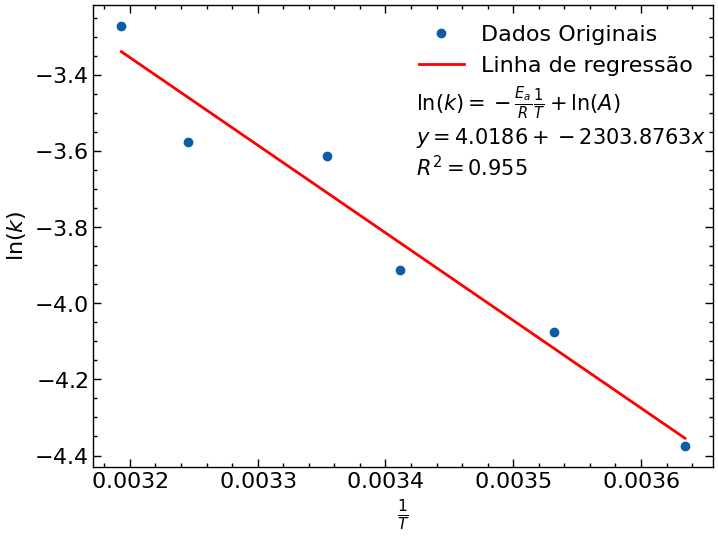
\includegraphics[width=0.8\textwidth]{ex2_grafico}
    \caption{Gráfico da linearização da equação de Arrhenius}
    \label{fig:ex2_grafico}
\end{figure}
E os seguintes valores para os parâmetros:
\begin{align}
    a &= \ln A = 4.014 \\
    b &= -\frac{E}{R} = 2301
\end{align}
Portanto, nosso valor da energia de ativação é \(E = 2301 \cdot 8.314 = 19130 \; \frac{J}{mol}\) e
nosso valor de \(A\) é \(A = \exp ^{4.014} = 55.368 \; \frac{1}{s}\). 
%────────────────────────────────────────────────────────────────────────────────────────────────────────────────────────────────────────────────────
%Começo do Capítulo 2 na apostila dele
\section{Reações de Pseudo-Primeira Ordem}
Seja uma reação qualquer, dada por
\begin{equation}
    \ch{A + B -> C }
\end{equation}
Onde a taxa de reação é dada por:
\begin{equation}
    \left( -r_A \right) = k C_A C_B
\end{equation} 
Reações de segunda ordem geram expressões bastantes complexas, bem mais que aquelas de primeira
ordem. Uma forma fácil de simplificação para resolução de exercícios é tratá-la como uma reação de
pseudo-primeira ordem, trabalhando com um grande excesso de um dos reagentes. \par

Supondo na reação enunciada acima que tivéssemos 0.5 mols de \(A\) e 100 mols de \(B\), ao final da
reação, a concentração de \(B\) quase não teria variação, podendo ser tratada como constante. Logo,
se tivermos um reator com volume \(V\), \(B\) teria uma concentração \(C_B = \frac{N_{B0} }{V}\).
Podemos definir uma constante pseudo-cinética, \(k^{\prime} \), dada por:
\begin{equation}
    k^{\prime} = k C_B 
\end{equation}
Podemos definir nossa velocidade para a reação de pseudo-primeira ordem como:
\begin{equation}
    \left( -r_A \right) = k^{\prime} C_A
\end{equation}
Essa aproximação só é válida se um dos reagentes exceder em pelo menos 20 vezes a concentração do
outro reagente.  \par
%────────────────────────────────────────────────────────────────────────────────────────────────────────────────────────────────────────────────────
\section{Equilíbrio Químico}
A diversas reações químicas que são reversíveis e para qual a velocidade de formação dos reagentes a
partir da formação dos produtos vai aumentando com o tempo, devido ao aumento da concentração dos
produtos. Seja a reação elementar dada por:
\begin{equation}
    \ch{A <=> B}
\end{equation}
Sabendo que a reação direta apresenta uma constate de velocidade \(k_d\) e a inversa uma constante
de velocidade \(k_i\). A par que a reação ocorre, a concentração de \(A\) diminui e a de \(B\)
aumenta. Isso faz com que se tenha uma variação de velocidade ao longo da reação, a par que as
concentrações vão mudando a velocidade muda proporcionalmente. \par

No equilíbrio, as velocidades de reação sao iguais, ou seja, a velocidade da reação direta é igual a
velocidade da reação inversa, portante, podemos afirmar que as concentrações se mantém constantes.
No estudo dessas reações, é importante saber como é a variação de um determinado reagente no meio
reacional. Na reação anteriormente mencionada, temos que o valor \(\left( -r_{A}  \right) \) é dado
por:
\begin{equation}
    \left( -r_{a} \right) = \left( -r_A \right)_d - \left( +r_A \right)_i 
\end{equation}

Onde temos que o reagente é consumido durante a reação direta e produzido durante a reação inversa.
Por estequiometria, temos que a taxa de produção de \(A\) na reação inversa é a mesma de consumo de
\(B\), logo podemos reescrever a equação acima como:
\begin{equation}
    \left( -r_{a} \right) = \left( -r_A \right)_d - \left( -r_B \right)_i 
\end{equation}
Onde, substituindo as equações de velocidade, temos:
\begin{equation}
    \left( -r_{a} \right) = k_d C_A - k_i C_B
\end{equation}
Para o equilíbrio, temos que \(\left( -r_{a} \right) = 0\), logo:
\begin{equation}
    \frac{k_d}{k_i} = \frac{C_{Be} }{C_{Ae} } = K_c
\end{equation}
Onde \(K_c\) é a constante de equilíbrio. Os índices \(e\) indicam que são as concentrações no
equilíbrio. \par
Assim, a constante de equilíbrio é determinada pelas concentrações de equilíbrio dos reagentes e
produtos. Para uma reação \(\ch{A + 2B <=> 3C + D}\), nossa constante de equilíbrio é dada por:
\begin{equation*}
    K_c = \frac{C_{Ce}^3 C_{De} }{C_{Ae} C_{Be}^2}
\end{equation*} 
Porém, essa relação só é válida para reações elementares, para reações não-elementares. Para a
reação não elementar abaixo, temos que:
\begin{equation}
    \ch{3ClO- <=> ClO3- + 2Cl-}
\end{equation}
A constante de equilíbrio é dada por:
\begin{equation}
    K_c = \frac{C_{ClO_3^-} C_{Cl^-}^2}{C_{ClO^-}^3}
\end{equation}
Porém, essa reação é composta de duas reações elementares, que são:
\begin{align*}
    \ch{2ClO- &<=>[k_1][k_{1,Inv}] ClO2- + Cl-}
    \ch{ClO2- + ClO- &<=>[k_2][k_{2,Inv}] ClO3- + Cl-}
\end{align*}
No equilíbrio, as velocidades das reações diretas e inversas são iguais, logo:
\begin{align*}
    k_1 C_{\ch{ClO}_{e}}^{2} = k_{1,Inv} C_{\ch{ClO2}_{e}} C_{\ch{Cl-}_{e}} \\
    k_2 C_{\ch{ClO2-}_{e}}C_{\ch{ClO-}_{e}} = k_{2,Inv} C_{\ch{ClO3-}_{e}} C_{\ch{Cl-}_{e}}
\end{align*}
Dividindo a primeira equação pela segunda, temos:
\begin{equation}
    \frac{k_1}{k_2} \frac{C_{\ch{ClO}_{e}}^{2}}{C_{\ch{ClO2-}_{e}}C_{\ch{ClO-}_{e}}} = \frac{k_{1,Inv}}{k_{2,Inv}} \frac{C_{\ch{ClO2-}_{e}} C_{\ch{Cl-}_{e}}}{C_{\ch{ClO3-}_{e}} C_{\ch{Cl-}_{e}}}
\end{equation}
Onde, isolamos as constantes de velocidade e as concentrações de equilíbrio, temos:
\begin{equation}
    \frac{k_1 k_2}{k_{1,Inv} k_{2,Inv}} = \frac{C_{\ch{ClO3-}_{e}}C_{\ch{Cl-}_{e}}}{C_{\ch{ClO2-}_{e}}}
\end{equation}
%────────────────────────────────────────────────────────────────────────────────────────────────────────────────────────────────────────────────────
\section{Reações em Fase Gasosa}
Para uma reação em fase gasosa elementar qualquer, temos:
\begin{equation}
    \ch{A + B -> C}
\end{equation}
Onde a velocidade de reação é dada por:
\begin{equation}
    \left( -r_A \right)^{\star} =k^{\star} P_A P_B
\end{equation}
Em termos das pressões parciais dos nossos gases. Poderíamos escrever em função da concentração,
também seria totalmente valido, porem, para gases, é mais comum trabalhar com pressão. \par

Nota-se também que os valores que seriam obtidos por \(\left( r_A \right) \) e \(\left( r_A
\right)^{\star} \) serão diferentes, similarmente como as constantes de velocidade \(k\) e
\(k^{\star} \) também são. \par

A constante \(k^{\star} \) é a constante de velocidade em termos de pressão parcial, existindo uma
correlação com \(k\) que dependerá da ordem de reação,. Se aplicarmos a equação de Clapeyron ao
reagente \(A\), temos:

\begin{align}
    P_A V &= n_A R T \\
    C_A &= \frac{n_A}{V} =  \frac{P_A}{RT} \\
\end{align}
O processo é o mesmo para o reagente \(B\). Substituindo na nossa equação de velocidade, temos:
\begin{align}
    \left( -r_A \right)^{\star} &= k^{\star} P_A P_B \\
    \left( -r_A \right)^{\star} &= k^{\star} C_A C_B \left( RT \right)^2 \\
    \frac{\left( -r_A \right)^{\star}}{RT} &= k^{\star} C_A C_B RT
    \frac{\left( -r_A \right)^{\star}  }{RT} &= \left( -r_A \right) 
\end{align}
Onde a relação entre as constantes de velocidade é \(k = k^{\star} RT\) válida para reações de
segunda ordem. Em fato, a depender da ordem, a formula geral para conversão é dada por
\begin{equation}
    k = k^{\star} \left( RT \right)^{n-1}
\end{equation}
Onde \(n\) é a ordem da reação. \par
%Fim da seção de reações em fase gasosa
%────────────────────────────────────────────────────────────────────────────────────────────────────────────────────────────────────────────────────
\section{Exercícios}
\subsection{Exercício 1}
A reação \ch{A + B -> C + D} foi estudada em laboratório e as concentrações dos reagentes foram
monitoradas ao longo do tempo, dando a seguinte tabela:
\begin{table}[H]
\centering
\begin{tabular}{c|c|c|c|c|c|c}
\toprule
Tempo (min) & 0 & 10 & 30 & 60 & 90 &  120 \\
 \midrule
 \(C_A\) \(\frac{mol}{L}\)  & 1 & 0.8 & 0.6 & 0.5 & 0.4 &  0.35 \\
 \(C_B\) \(\frac{mol}{L}\)  & 20 & 19.8 & 19.6 & 19.5 & 19.4 &  19.35 \\
\bottomrule
\end{tabular}
\caption{Tempo e concentração dos Reagentes}
\label{tab:cap2_ex1_tabela}
\end{table}
Sabendo que ela é elementar e possui \(k = 2.5 \; \frac{mol}{L \cdot  min}\), verifique se ela pode
ser tratada como de pseudo-primeira ordem. Faça o grafico de \(\left( -r_A \right) \) por \(t\)
\subsection{Resolução}
Vamos determinar as reações de velocidade para o reagente \(A\), considerando como reação de segunda
ordem e pseudo-primeira ordem, respectivamente:
\begin{align}
    \left( -r_A \right) &= 2.5 \cdot C_A \cdot C_B \\
    \left( -r_A \right) &= 2.5 \cdot C_A \cdot 20 = 50 \cdot C_A
\end{align}
O gráfico é feito pelo python pelo seguinte código:
\begin{minted}[linenos]{python}
import numpy as np
import matplotlib.pyplot as plt

t = np.array([0, 10, 30, 60, 90, 120])
Ca = np.array([1, 0.8, 0.6, 0.5, 0.4, 0.35])
Cb = np.array([20, 19.8, 19.6, 19.5, 19.4, 19.35])

ra_seg = 2.5 * Ca * Cb
ra_pse = 50 * Ca

fig = plt.figure()
ax = fig.add_subplot()
ax.plot(t, ra_seg, 'o', label='Segunda Ordem')
ax.plot(t, ra_pse, 'o', label='Pseudo-Primeira Ordem')
plt.xlabel(r'$t \; (min)$')
plt.ylabel(r'$\left( -r_A \right) \; \frac{{mol}}{{L \cdot min}}$')
plt.legend()
plt.show()
\end{minted}
Resultando no seguinte gráfico
\begin{figure}[H]
    \centering
    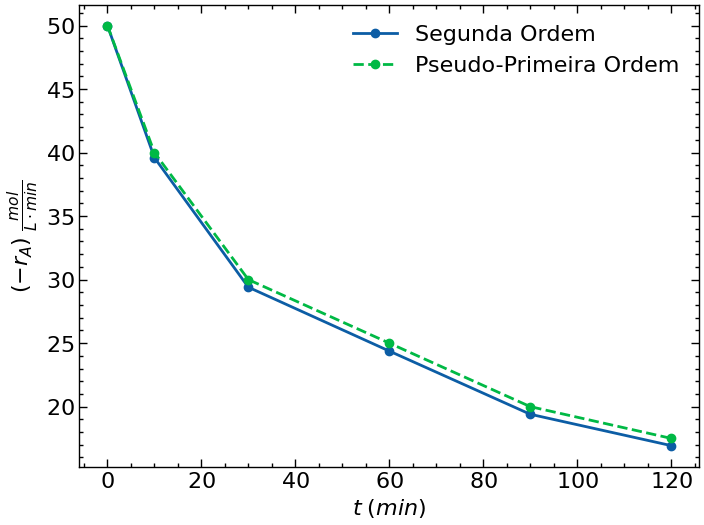
\includegraphics[width=0.8\textwidth]{cap2_ex1_grafico}
    \caption{Gráfico de \(\left( -r_A \right) \) por \(t\)}
    \label{fig:cap2_ex1_grafico}
\end{figure}
%Fim da resolução do exercício 1
%────────────────────────────────────────────────────────────────────────────────────────────────────────────────────────────────────────────────────
\subsection{Exercício 2}
Seja a reação não elementar \ch{H2O2 + H+ + I- <=> H2O + HOI}. Sabendo que ela pode ser representada
pelos seguintes passos elementares:
\begin{align*}
    \ch{H+ + I- &<=>[k_1][k_{1,Inv}] HI} \\
    \ch{HI + H2O2 &<=>[k_2][k_{2,Inv}] H2O + HOI} \\
\end{align*}
Onde \(k_1 = 0.0023, \; K_{1, Inv} = 0.44, \; k_2 = 1.03 \cdot 10^{-4}, \; k_{2, Inv} = 22 \), todas
em \(\frac{L}{mol \cdot min}\). Determine o valor de \(k_{c} \) 
\subsection{Resolução}
No equilíbrio, nossas reações inversas e diretas tem a mesma taxa de reação, logo:
\begin{align*}
    k_1 C_{\ch{H+}_{e}} C_{\ch{I-}_{e}} &= k_{1,Inv} C_{\ch{HI}_{e}} \\
    k_2 C_{\ch{HI}_{e}} C_{\ch{H2O2}_{e}} &= k_{2,Inv} C_{\ch{H2O}_{e}} C_{\ch{HOI}_{e}} \\
\end{align*}
Multiplicando as equações, vamos ter:
\begin{align*}
    k_1 k_2 C_{\ch{H+}_{e}} C_{\ch{I-}_{e}} C_{\ch{HI}_{e}} C_{\ch{H2O2}_{e}} &= k_{1,Inv} k_{2,Inv} C_{\ch{HI}_{e}} C_{\ch{H2O}_{e}} C_{\ch{HOI}_{e}} \\
    \frac{k_1 k_2}{k_{1,Inv} k_{2,Inv}} &= \frac{C_{\ch{H2O}_{e}} C_{\ch{HOI}_{e}}}{C_{\ch{H+}_{e}} C_{\ch{I-}_{e}} C_{\ch{HI}_{e}} C_{\ch{H2O2}_{e}}} \\
    K_c &= \frac{C_{\ch{H2O}_{e}} C_{\ch{HOI}_{e}}}{C_{\ch{H+}_{e}} C_{\ch{I-}_{e}} C_{\ch{H2O2}_{e}}} \\
\end{align*}
Ou seja, nossa constante de equilíbrio tem valor de
\begin{equation*}
    k_{c} = \frac{1.03 \cdot 10^{-4} \cdot 0.0023}{0.44 \cdot 22} = 2.44731 \cdot 10^{-8}
\end{equation*}
%Fim da resolução do exercício 2
%────────────────────────────────────────────────────────────────────────────────────────────────────────────────────────────────────────────────────
\subsection{Exercício 3}
A reação hipotética \ch{A => 2B} com um \(k = 278 \; \frac{L^{2} }{mol ^{2} s}\). Escreva a equação
de velocidade para essa reação em termos de concentração e em termos de pressão parcial. 
\subsection{Resolução}
Primeiramente será necessário realizar análise dimensional da nossa concentração.
\begin{align*}
    \left( -r_A \right) &= k C_A^n \\
    \left( \frac{mol}{L \cdot s} \right) &= \left( \frac{L^{2}}{mol ^{2} s}  \right)  \left( \frac{mol^{3}}{L^{3} } \right)      
\end{align*}
Portanto, nossa concentração tem unidade de \(\frac{mol^{3} }{L^{3} }\), com \(n = 3\). NOssa reação
é de terceira ordem. Portanto, para achar \(k^{\star} \) aplicamos a formula
\begin{align*}
    k &= k^{\star} \left( RT \right)^{n-1} \\
    278 &= k^{\star} \left( 8.314 \cdot 298 \right)^{3-1} \\
    k^{\star} &= 0.454 \; \frac{1}{atm^{2} \cdot s}
\end{align*} 
Portanto, nossa equação fica
\begin{equation*}
    \left( -r_A \right)^{\star} = 0.454 \cdot P_A^3
\end{equation*}
%Fim da resolução do exercício 3
%────────────────────────────────────────────────────────────────────────────────────────────────────────────────────────────────────────────────────
%Inicio do capitulo 3 na apostila dele
%to do
\section{Estequiometria Cinética-Conversão}
A conversão, geralmente denotada pela letra \((X_n)\) indica a quantidade que foi reagida em relação
a quantidade inicial que tínhamos. Será utilizado a letra \(A\) para o reagente limitante. Portanto,
para o limitante, temos \(X_A\) de conversão, variando de \(0 \to 1\). Considere a reação
genérica \ch{aA + bB -> cC + dD}, ocorrendo em batelada em um determinado reator. Indicamos o índice
\(0\)  como sendo para o instante inicial. Ou seja, no instante inicial teríamos \(n_{A0} \) mols de
\(A\), \(n_{B0} \) mols de \(B\), \(n_{C0} = 0\) mols de \(C\) e \(n_{D0} = 0\) mols de \(D\). \par

\begin{figure}[ht]
	\centering
	\caption{}
	%\incsvg{path/}{path/file}
	\incsvg{Materias/Imagens}{Materias/Imagens/Reator_Batelada}\\
	\label{fig:Reator_Batelada}
\end{figure}

Quando não colocamos índice, estamos indiciando que é num instante \(t\) qualquer de tempo. A
conversão do nosso reagente limitante é dada por:
\begin{equation}
    X_A = \frac{n_{A0} - n_A}{n_{A0} }
\end{equation}
%────────────────────────────────────────────────────────────────────────────────────────────────────────────────────────────────────────────────────
\subsection{Tabela Estequiométrica}
Considerando os coeficientes da reação genérica anterior, temos a seguinte tabela:
\begin{table}[H]
\centering
\begin{tabular}{c|c|c|c|c|c}
\toprule
 & \ch{aA} & \ch{bB} & \ch{->} & \ch{cC} &  \ch{dD} \\
 \midrule
 Início & \(N_{A0}\)  & \(N_{B0}\)  &  & \(N_{C0}\)  &  \(N_{D0}\)  \\
 Variação & \(-N_{A0} X_A\)  & \(-\frac{b}{a}N_{A0}X_A\)  &  & \(\frac{c}{a}N_{A0}X_A\)  & \(\frac{d}{a} N_{A0}X_A\)   \\
 Restante &  \(N_{A0} - N_{A0} X_A\)  & \(N_{B0} - -\frac{b}{a}N_{A0}X_A\)  &  & \(N_{C0} - \frac{c}{a}N_{A0}X_A\)  &  \(N_{D0} - \frac{d}{a} N_{A0}X_A \)  \\
\bottomrule
\end{tabular}
\caption{Tabela Estequiométrica Genérica}
\label{tab:tablea_estequiometrica}
\end{table}

Para um instante \(t\) qualquer, temos a seguinte fórmula para a quantidade presente no reator:
\begin{equation}
    N_{i} = N_{A0} \left( \frac{N_{i0} }{N_{A0} } + \gamma_i \frac{i}{a}X_A \right)  
\end{equation}
Onde \(i\) é o índice do reagente ou produto e \(\gamma_i\) é um operador que possui valores dados
abaixo
\begin{equation}
    \begin{dcases}
    1, &\text{ se } \text{Produto} ;\\
    -1, &\text{ se } \text{Reagente} ;\\
    \end{dcases}
\end{equation}

Importante que essas formulas são validas para qualquer tempo, porém, nãos oferecem relação nenhuma
para saber o tempo da reação.\par
%────────────────────────────────────────────────────────────────────────────────────────────────────────────────────────────────────────────────────
\section{Variações de Concentração}
Como o número de mols varia com tempo, não é nada distante imaginar que a concentração também
variará em função do tempo. Basta pegar pela própria definição de concentração \(C_A =
\frac{N_A}{V}\). Vale ressaltar que essa formula apenas é válida quando todas as espécies estão
igualmente distribuídas no volume do reator. \par

\subsection{Reações a Volume Constantes}  
Se conduzirmos nossa reação em um reator fechado e de paredes rígidas, podemos admitir que o volume
se manterá constante. Similarmente, se fizermos uma reação apenas com fases líquidas, não é muito
distante pensar que o volume se manterá constante. Sendo assim, podemos considerar \(V = V_0\), ou
seja, nossas equações de concentração ficam:

\begin{equation}\label{eq:cap3_concentracao_volume_fixo}
    C_i = C_{A0} \left( \frac{N_{i0}}{N_{A0} } + \gamma_i \frac{i}{a}X_A \right)  
\end{equation}

Geralmente, para produtos, temos que \(N_{C0} = N_{D0} = 0 \), podendo simplificar um pouco nossas
equações. 

\subsection{Reações a Volume Variável}
Quando temos reações a volume variável, ou seja, em fases gasosas, reator contínuo ou em batelada de
parede móvel, temos que a concentração varia com o tempo. Podemos considerar, em fases gasosa, o
volume reacional com função do número  total de mols através da equação de Clapeyron:

\begin{equation}
    V = \frac{n R T}{P} = \frac{\left( N_A + N_B + N_C + N_D \right) RT}{P}
\end{equation}

Podemos simplificar essa equação, substituindo os valores de \(N_i\) em função de \(X_A\), temos:

\begin{equation}
    V = \left[N_{A0} \left( 1 + \frac{N_{B0} }{N_{A0}} + \frac{N_{C0} }{N_{A0}} + \frac{N_{D0} }{N_{A0}}\right) + N_{A0}\frac{d+c-b-a}{a}X_A \right] \frac{RT}{P}
\end{equation}

Definindo a grandeza 

\begin{equation}
    y_{A0} = \frac{N_{A0} }{N_{T0}}
\end{equation}

Onde \(N_{T0} = N_{A0} + N_{B0} + N_{C0} + N_{D0} \) é o número total de mols no instante inicial.
Substituído de volta na equação anterior, temos:

\begin{equation}
    V = \left( N_{T0} + y_{A0} N_{T0} \frac{d+c-b-a}{a}X_A \right) \frac{RT}{P}
\end{equation}

A fração de conversão volumétrica é dada por:

\begin{equation}
    \varepsilon _A = y_{A0} \delta  
\end{equation}

Onde \(\delta = \frac{d+c-b-a}{a}\). A fração de conversão volumétrica é também conhecida como o
fator  de expansão, indicando o quanto o sistema se expande ou contrai durante a reação. \par

Substituindo de volta na equação anterior, temos:

\begin{equation}
    V = \left( 1 + y_{A0} \delta X_A \right) N_{T0} \frac{RT}{P}    
\end{equation}

Podemos utilizar a equação de Clapeyron para a condição inicial

\begin{equation}
    N_{T0} = \frac{P_0 V_0}{RT_0}
\end{equation}

Com isso, temos:

\begin{equation}
    V = \left( 1 + \varepsilon_A X_A \right) \frac{P_{0} T }{P T_0}
\end{equation}

Com isso, para nossas concentrações, temos:

\begin{equation}\label{eq:cap3_concentracao_volume_variavel}
    C_i = \frac{C_{A0}\left( \frac{N_{i0}}{N_{A0} } +\gamma_i \frac{i}{a}X_A\right)}{\left( 1 + \varepsilon_A X_A \right) \frac{P_0T}{PT_0} }
\end{equation}
%────────────────────────────────────────────────────────────────────────────────────────────────────────────────────────────────────────────────────
\section{Exercícios}
\subsection{Exercício 1}
A reação \ch{H2 + Cl2 -> 2HCl} é realizada em fase gasosa a 5 atm em um reator de paredes móveis com
concentrações iniciais de \(C_{H2} = 3 \; \frac{mol}{L} \) e \(C_{Cl2} = 4 \; \frac{mol}{L} \).
Determine
\begin{enumerate}
    \item O reagente limitante \label{item:cap3_ex1_item1}
    \item A concentração de \ch{Cl2} no tempo de meia vida da reação \label{item:cap3_ex1_item2}
    \item A pressão parcial de \ch{HCl} apos \(70 \%\) de conversão \label{item:cap3_ex1_item3}
    \item {Se \(73 \; \frac{g}{L}\) de \ch{HCl} estiverem presentes no início da reação, qual sera
    sua conversão se sua concentração atingir \(146 \; \frac{g}{L}\) \label{item:cap3_ex1_item4}}
\end{enumerate}
\subsection{Resolução}
\subsubsection{Item \ref{item:cap3_ex1_item1}}
Para determinar qual irá ser o limitante, vamos analisar a quantidade alimentada \textit{vs} a
quantidade estequiométrica necessária para a reação. Temos que:
\begin{equation*}
    \ch{1H2 + 1 Cl2 -> 2HCL}
\end{equation*}
Temos que nossas quantias estequiométricas são 1 mol de \ch{H2} para 1 mol de \ch{Cl2}. Portanto,
aquele com menor quantia será o limitante, no nosso caso, será o \ch{H2}.

\subsubsection{Item \ref{item:cap3_ex1_item2}}

Conforme estabelecido \(A\) é tratado como o reagente limitante. Como foi dito que, a reação é
gasosa e em paredes móveis, temos que usar a equação \refeq{eq:cap3_concentracao_volume_variavel}.
Portanto, para o \ch{Cl2}, temos:

\begin{equation*}
    C_{Cl2} = \frac{C_{A0} \left( \frac{N_{Cl20}}{N_{A0} } - \frac{1}{1}X_A \right)}{\left( 1 + \varepsilon_A X_A \right) \frac{P_0T}{PT_0} }
\end{equation*}

Porém, temos que

\begin{align*}
    \delta &= \frac{c - b - a}{a}\\
    &= \frac{2 - 1 - 1}{1}
    &= 0
\end{align*}

Considerando nossa reação como isotérmica e à pressão constante, nossa equação se reduz a

\begin{equation*}
    C_{Cl2} = C_{A0} \left( \frac{N_{Cl20}}{N_{A0} } - \frac{1}{1}X_A \right)
\end{equation*}

Onde o tempo de meia vida é dado por \(X_A = 0.5\). Substituindo os valores, temos:

\begin{align*}
    C_{Cl2} &= 3 \left( \frac{4}{3} - \frac{1}{1} \cdot 0.5 \right) \\
    &= 2.5 \; \frac{mol}{L}
\end{align*}

\subsubsection{Item \ref{item:cap3_ex1_item3}}

Fazendo as mesmas correlações para o produto, nossa formula se reduz a:

\begin{equation*}
    C_{HCl} = C_{A0} \left( \frac{N_{HCl0}}{N_{A0}} + \frac{2}{1}X_A \right)
\end{equation*}

Multiplicando nossa equação por \(RT\), temos:

\begin{align*}
    C_{HCl} = C_{A0} RT \left( \frac{N_{HCl0}}{N_{A0}} + 2 X_A \right)
    P_C = P_{A0} \left( \frac{N_{HCl0}}{N_{A0}} + 2 X_A \right)
\end{align*}

Sabendo que \(P_{A0}  = y_{A0} P\), temos

\begin{align*}
    P_C = P_{A0} \left( \frac{N_{HCl0}}{N_{A0}} + 2 X_A \right)
\end{align*}

% \chapter{Laboratorio de Engenharia Quimica}
\section{LEQ1}  
\subsection{Experimento 1}

% \chapter{Controle de Processos Químicos}
\label{chap:cpq}
\section{Introdução}
\label{sec:cpq-intro}
Esse professor é maluco da cabeça, ele não segue nenhuma linha de raciocínio então o que será
escrito aqui é apenas uma tentativa de organizar as ideias dele. \par

Imaginemos que tenhamos uma planta com uma entrada mássica com valor \(w\), de um fluido qualquer.
Ele possui uma temperatura \(T_i(t)\) de entrada. Dentro do tanque de armazenamento, existe um
aquecedor, que aquece o fluido até uma temperatura \(T\), qualquer. Se estivermos um regime
estacionário, nossa vazão mássica também sera \(w\). Queremos que nosso regime seja estacionário,
logo, que a temperatura de estado estacionário, \(T_{is}\), que essa será a mais importante de
entendermos. Se formos colocar em variável desvio, teremos que \(T_i(t) = T_i(s) - T_{is}\). \par

Na nossa saída do tanque, nosso líquido terá uma temperatura \(T_{s} = T_R\), ou em variável desvio
\(T^{\prime} (t) = T(t) - T_R\). \footnote{O linha (\(^{\prime} \) ), geralmente utilizada para derivada, nesse caso é
para significar variável desvio, porém, nem sempre isso será verdade.}

%Honestamente é preferível a morte

Se tivermos uma introdução de uma pertubação do estilo degrau, teremos que \(T_i(t) = T_i(s) -
T_{is} + \Delta T_i\), onde
\begin{equation}
    \Delta T_i = \begin{cases}
        T_{is} , & t < 0 \\
        T_{is} + \Delta T_i, & t \geq 0
    \end{cases}
\end{equation}
Vamos querer sempre fazer com que essa variação seja a mais abrupta possível, para que se tenha nos
aproximar o máximo possível de um degrau. Mas claro, que vamos ter um tempo de resposta, que terá um
erro associado, ou seja, para uma dada equação, temos
\begin{align}
    \dot{q}(t) &= \dot{q}_s + k_{c} e(t)\\
    \dot{q}(t) - \dot{q}_s = k_{c} e(t) &= \dot{Q}(t)\\
    k_{c} &> 0\\
    e(t) &= T_R - T(t)\\
\end{align}
Para essa equação em particular, estamos tratando de energia, calor. Se formos fazer um balanço de
energia, temos
\begin{align}
    \dot{q}(t) - w_{c} \left( T(t) - T_{i} (t) \right) = \rho v_{c} \frac{\mathrm{d}T(t)}{\mathrm{d}t}  
\end{align}
Onde em facilmente é apenas a taxa que entra é a taxa que sai.
\section{Transformada de Laplace}
A transformada de Laplace é uma das mais importantes ferramentas matemáticas para a análise de
sistemas dinâmicos. Ela é uma ferramenta que nos permite transformar uma equação diferencial em uma
equação algébrica. Ela é definida como:
\begin{equation}\label{eq: equacao de laplace}
    \mathcal{L} \left\{ f(t) \right\} = F(s) = \int_{0}^{\infty} f(t) e^{-st} \mathrm{d}t
\end{equation}
Onde \(s\) é um número complexo. A transformada de Laplace é uma transformada linear, ou seja,
\begin{equation}
    \mathcal{L} \left\{ a f(t) + b g(t) \right\} = a F(s) + b G(s)
\end{equation}
A transformada de Laplace é uma transformada de uma função de tempo para uma função de frequência,
geralmente com a variável \(s\). Vamos ver alguns exemplos.
\subsection{Exemplo 1}
Seja o PVI dado por
\begin{align}
    \begin{dcases}
        2 \frac{\mathrm{d}\xi (t)}{\mathrm{d}t} + \xi (t) &= 1;\\
        \xi (0) &= 0\\
    \end{dcases}
\end{align}
Resolva esse PVI utilizando a transformada de Laplace. \par
\textbf{Solução:} Aplicando a transformada de Laplace na equação diferencial, temos
\begin{align}
    \mathscr{L} \left\{ 2 \frac{\mathrm{d}\xi (t)}{\mathrm{d}t} + \xi (t) &= 1 \right\}\\
    2 \mathscr{L} \left\{ \frac{\mathrm{d}\xi (t)}{\mathrm{d}t} \right\} + \mathscr{L} \left\{ \xi (t) \right\} &= \mathscr{L} \left[ 1 \right]\\
    2 s \left[\mathscr{L} \left\{ \xi (t) \right\} - \xi (0)\right] + \mathscr{L} \left\{ \xi (t) \right\} &= \frac{1}{s}\\
    2 s \left[\mathscr{L} \left\{ \xi (t) \right\} - 0\right] + \mathscr{L} \left\{ \xi (t) \right\} &= \frac{1}{s}\\
    \mathscr{L} \left\{ \xi (t) \right\} \left( 2s + 1 \right) &= \frac{1}{s}\\
    \mathscr{L} \left\{ \xi (t) \right\} &= \frac{1}{s \left( 2s + 1 \right)}\\
    \mathscr{L} \left\{ \xi (t) \right\} &= \frac{1}{s} - \frac{2}{2s + 1}
\end{align}
%Falta aplicar a inversa
%────────────────────────────────────────────────────────────────────────────────────────────────────────────────────────────────────────────────────
\subsection{Exemplo 2}
Seja o PVI dado por
\begin{align}
    \begin{dcases}
        \frac{\mathrm{d}^2  T(t)}{\mathrm{d}t^2} + 2 \frac{\mathrm{d} T(t)}{\mathrm{d}t} + T(t) = 2 \\
        T(0) = 3\\
        \frac{\mathrm{d} T(t)}{\mathrm{d}t} \bigg|_{t=0} = 1\\
    \end{dcases}
\end{align}
Resolva esse PVI utilizando a transformada de Laplace. \par
\textbf{Solução:} Aplicando a transformada de Laplace na equação diferencial, temos
\begin{align}
    \mathscr{L} \left\{ \frac{\mathrm{d}^2  T(t)}{\mathrm{d}t^2} + 2 \frac{\mathrm{d} T(t)}{\mathrm{d}t} + T(t) = 2 \right\}\\
    \mathscr{L} \left\{ \frac{\mathrm{d}^2  T(t)}{\mathrm{d}t^2} \right\} + 2 \mathscr{L} \left\{ \frac{\mathrm{d} T(t)}{\mathrm{d}t} \right\} + \mathscr{L} \left\{ T(t) \right\} &= \mathscr{L} \left\{ 2 \right\}\\
    s^2 \mathscr{L} \left\{ T(t) \right\} - s T(0) - \frac{\mathrm{d} T(t)}{\mathrm{d}t} \bigg|_{t=0} + 2 s \mathscr{L} \left\{ T(t) \right\} - T(0) + \mathscr{L} \left\{ T(t) \right\} &= \frac{2}{s}\\
    s^2 \mathscr{L} \left\{ T(t) \right\} - 3 s + 1 + 2 s \mathscr{L} \left\{ T(t) \right\} - 3 + \mathscr{L} \left\{ T(t) \right\} &= \frac{2}{s}\\
    \left( s^2 + 2s + 1 \right) \mathscr{L} \left\{ T(t) \right\} &= \frac{2}{s} + 3 s - 4\\
    \left( s + 1 \right)^2 \mathscr{L} \left\{ T(t) \right\} &= \frac{2}{s} + 3 s - 4\\
    \mathscr{L} \left\{ T(t) \right\} &= \frac{2}{s \left( s + 1 \right)^2} + \frac{3 s - 4}{\left( s + 1 \right)^2}\\
\end{align}
% Faltar aplicar a inversa
%────────────────────────────────────────────────────────────────────────────────────────────────────────────────────────────────────────────────────
\subsection{Exemplo 3}
Seja o PVI dado por


\end{document}
